\startchapter{Evaluation of Word Vectors using BrainBench V2.0}
\label{chapter:newsol}

The previous chapter discussed in detail about major contributions made in the field of study of representations of language. It also explained in depth about various Distributional Semantic models (DSM) or word vectors trained on text corpora and how Computational linguists use these models to study semantic representation in the human brain. The previous chapter also discussed \textit{BrainBench}- a system designed to test, evaluate and benchmark word vector models using brain data \cite{BrainBench2016}. \textit{BrainBench} reported comparable performance to other systems which evaluate and benchmark DSM's.

However, BrainBench tests include just 60 concrete nouns. Another limitation is that the tests do not include any abstract nouns. Moreover, the tests are derived from only two dataset sources (a fMRI and a MEG) and based on one language (English). Considering that DSM's are available in multiple languages and not including brain data from other language sources as a part of BrainBench tests is a limitation. 

To address these limitations, we release the second iteration of BrainBench (V2.0) which introduces two new datasets (a fMRI and an EEG dataset collected from Italian participants) to BrainBench tests. This addition improves the coverage of the tests from 60 words to 190 words. The Italian fMRI introduces abstract nouns to the test suite. We also evaluate the performance of word vectors trained on non-English corpora using our Italian brain dataset. Then we compare the performance of word vectors on abstract nouns and concrete nouns separately. 

Traditionally, EEG data was not recommended for studying semantics in Brain due to its weak Signal to Noise ratio (SNR). However, the work of Murphy et al. \cite{MurphyEEG} provided strong argument that EEG dataset along with semantic models is suitable for studying semantics in the brain. The results of our experiments with EEG dataset further reinforces this argument. EEG has higher temporal resolution and makes it ideal for exploring word comprehension and semantic representation in the brain. EEG is more portable and much cheaper as compared to fMRI, making it suitable for experiments.


Anderson et al. studied the performance of the performance of image-based semantic models against anatomical regions in human brain \cite{andersonBrainEyes}. However, the semantic models and the methodology used in our study are different to their study. We incorporate into BrainBench the ability to study word vector performance across the various anatomical region in the human brain. The methodology is discussed in detail in the section \textit{Evaluation of DS models against anatomical brain region} of this chapter.

The contributions to BrainBench addressed by this chapter are summarized below (\textit{Contribution A}).

\begin{itemize}

\item {Introduction of abstract nouns into the BrainBench tests and evaluation of the performance of various word vectors on abstract nouns.}
\item{Addition of Italian Brain data into BrainBench and study of the performance of non-English word vectors.}
\item {Addition of an EEG dataset to BrainBench.}
\item {The study of the performance of word vectors across various brain regions using brain Atlas mapping data collected using fMRI.}
\end{itemize}

\section{Brain Datasets}
%Give a three line Introduction
In this section, we discuss in detail about the four brain datasets that constitute the  BrainBench test suite. We primarily focus on the data collection techniques, concept selection and brain signal preprocessing for each of the below datasets.

\subsection{English fMRI}

The first major work in the study of semantics in the human brain using corpus-based semantic models was conducted by Mitchell et al. in 2008~\cite{Mitchell1191}. Nine right-handed participants were presented with 60 concrete nouns from 12 different semantic categories as listed under Table:~\ref{DataScienceFMRI} and their brain signals were recorded using a Siemens  Allegra 3.0T MRI scanner. The stimulus was presented in the form of line drawings and label text on the screen, and the participants were asked to imagine properties of the concepts presented. The set of 60 concepts were presented six times in random order resulting in 360 stimuli per participant. All the participants were native English speakers.

fMRI uses strong magnetic fields and radio waves to measure the changes in the blood flow in the brain to detect areas of activity. fMRI records blood flow changes in small 3D volume patches throughout the brain. These 3D volume patches are called as voxels. The number of voxels depends on the shape and size of a person's brain and average there were 20000 voxels per participant in this dataset. 

The fMRI signals collected from the study were preprocessing using the Statistical Parametric Mapping software (SPM2), corrected for head motion, linear trends. It was then spatially normalized into Montreal Neurological Institute space (MNI) and resampled to 3mm x 3mmx 6mm voxels. The dataset was then reshaped to words * voxels format (denoted as $w * v$)  and used for BrainBench tests. 

\begin{table}[t]
\centering

\begin{tabular}{|l|l|l|l|l|l|}
\hline
Category         & Word 1    & Word 2  & Word 3       & Word 4    & Word 5      \\ \hline
animals          & bear      & cat     & cow          & dog       & horse       \\ \hline
body parts       & arm       & eye     & foot         & hand      & leg         \\ \hline
buildings        & apartment & barn    & church       & house     & igloo       \\ \hline
building parts   & arch      & chimney & closet       & door      & window      \\ \hline
clothing         & coat      & dress   & pants        & shirt     & skirt       \\ \hline
furniture        & bed       & chair   & desk         & dresser   & table       \\ \hline
insects          & ant       & bee     & beetle       & butterfly & fly         \\ \hline
kitchen utensils & bottle    & cup     & glass        & knife     & spoon       \\ \hline
man made objects & bell      & key     & refrigerator & telephone & watch       \\ \hline
tools            & chisel    & hammer  & pliers       & saw       & screwdriver \\ \hline
vegetables       & carrot    & celery  & corn         & lettuce   & tomato      \\ \hline
vehicles         & airplane  & bicycle & car          & train     & truck       \\ \hline
\end{tabular}
\caption{The concepts studied using fMRI and MEG technology.}
The concepts studied by Mitchell et al.~\cite{Mitchell1191} and Sudre et al.~\cite{SUDRE2012451} using their experiments with fMRI and MEG respectively.
\label{DataScienceFMRI}
\end{table}

\subsection{English MEG}

In 2012, Sudre et al.~\cite{SUDRE2012451} investigated the flow of perceptual and semantic information in the brain by studying neural activities captured using Magnetoencephalography (MEG). MEG is a neuroimaging technique which captures the magnetic field changes produced by electric currents in the human brain. MEG has high temporal resolution and could be used to study changes in brain activity over time.

Nine right-handed participants were asked to answer 20 questions about 60 concrete concepts presented as line drawings on the screen. These concepts were the same as the ones studied by Mitchell et al.~\cite{Mitchell1191}  and listed under Table:~\ref{DataScienceFMRI}. In their experiment, a question was presented first to the participants followed by the 60 concrete concepts presented in random order. The participant responded with a \textit{yes or no} for each concrete noun. The experiments were repeated for a total of 20 questions resulting in 20 presentations per concept. The questions were on some properties of the concept such as \textit{was it alive?, Can you pick it up?} etc. All the participants were native English speakers.

The MEG data were recorded using an Elekta Neuromag device which has a total of 306 channels. The sampling was done at 200Hz, and MEG recording for each concept was 800ms long. The recorded data were preprocessed using Signal Space Separation method (SSS)~\cite{SSS} and low-pass filtered to 50Hz to remove line noise. The artifacts due to head movement, eye movements and blinking, and MEG sensor failures were subsequently removed using Signal Space Projection method ~\cite{SSP}. The data were then reshaped to $w*s*t$ format (words * sensors * time). Each data point in the matrix $s*t$ depicts the electrical activity collected from a sensor $s_i$ at time $t_j$. For simplicity, we would continue to call these data points as voxels throughout this thesis. The data is then mean normalized and used for our experiments.

\subsection{Italian fMRI}
This dataset was released as part of the experiments conducted by Anderson et al. to study the varying degree of concreteness in taxonomic categories in human brain using fMRI \cite{AndersonConcreteness}. Brain signal was collected from nine native Italian speakers viewing 70 concepts on a screen and imagining it. The 70 concepts selected were from two domains \textit{music} and \textit{law}. Moreover, these 70 concepts were organized into 7 Taxonomic categories (Attribute, Communication, Event, Social Role, Tool, Location and Urabstracts) using MultiWordNet~\cite{ItalianWordNet} (the Italian version of WordNet~\cite{wordnet})~ resulting in 70 stimuli with ten concepts from each taxonomic categories. Music and law domains had five words each within each taxonomic category. The concept selection was made in such a way that there was a varying degree of concreteness with the tool being the most concrete and Urabstracts being the most abstract taxonomic category. 

\begin{figure}[!t]
\centering
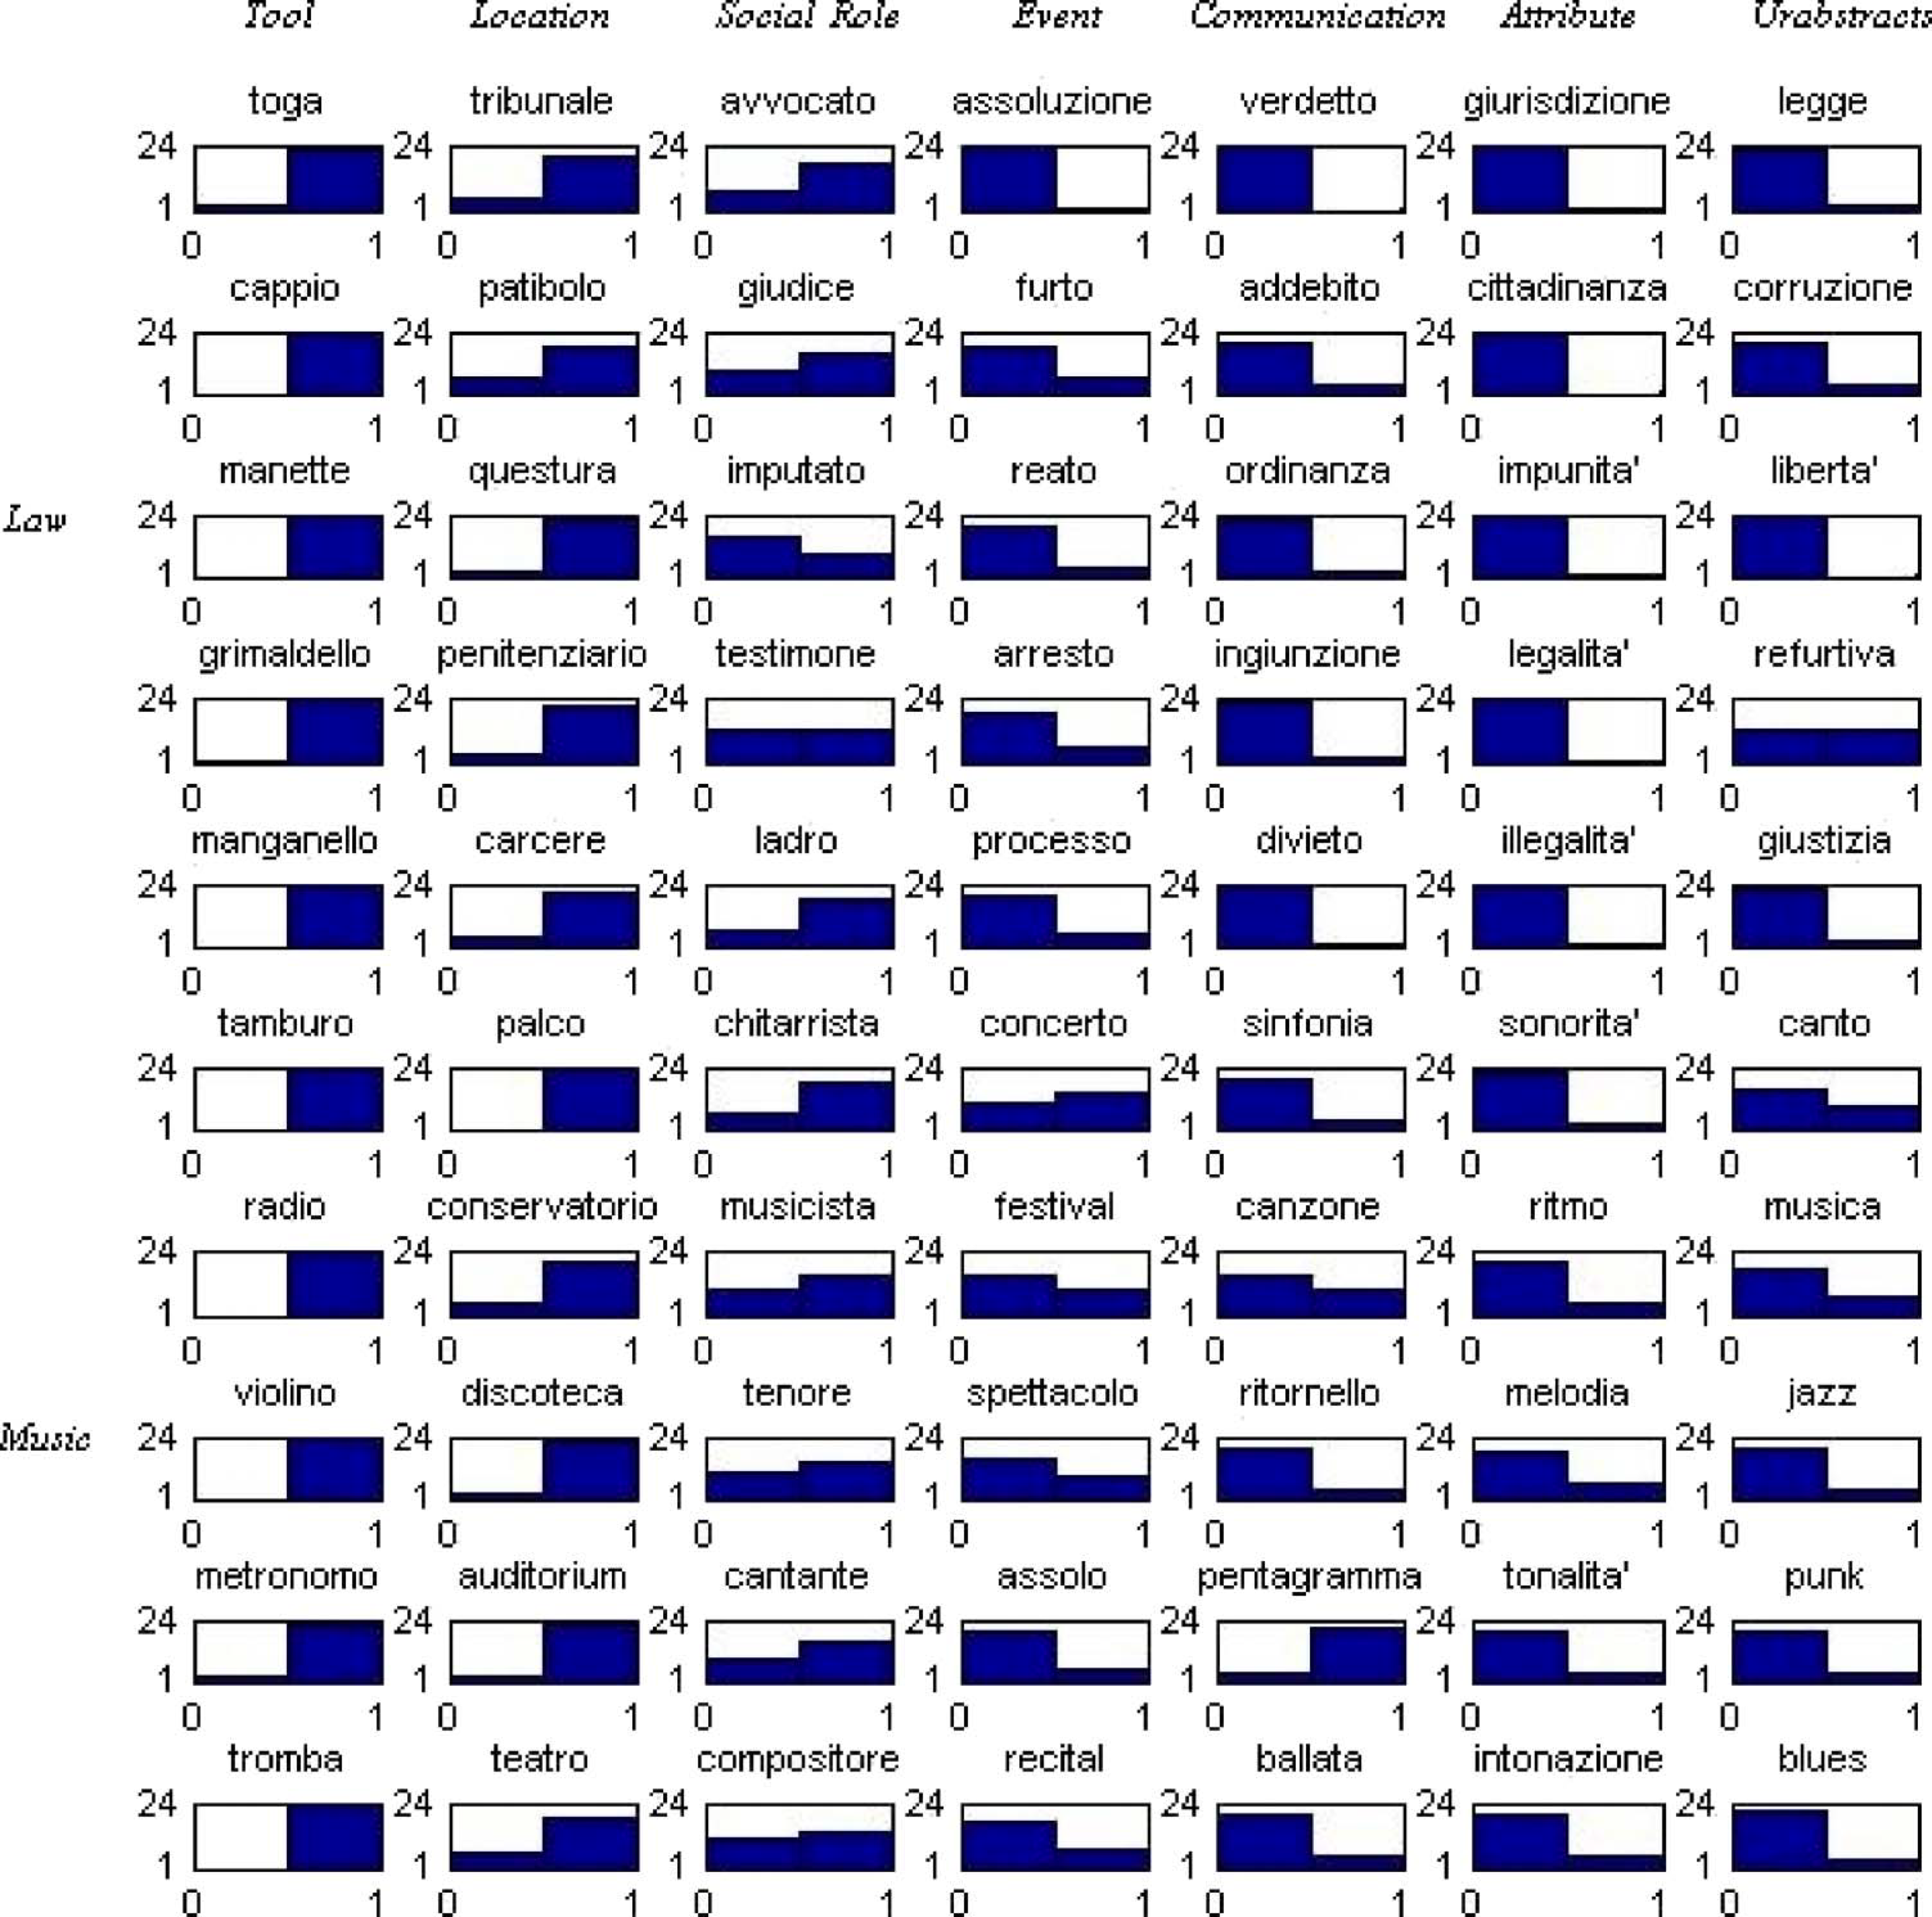
\includegraphics[width=12cm, height=12cm]{Figures/concreteness}
\caption{Word Norming Results for Concepts in Italian fMRI}
\label{ItalianFMRI}
70 concepts above organized into 7 Taxonomic categories and 2 Domains (music and law). The concreteness rating was assigned using word norming technique \cite{Barca2002WordNT} where 24 native Italian speakers were asked to rate the 70 concepts on a concreteness scale of 1 (highly abstract) to 7 (highly concrete). The collected data was binarized as concrete =1 and abstract =0. The y-axis indicates the rating of each of 24 participants.\\Image source: Anderson et al.,2014~\cite{AndersonConcreteness}.
\end{figure}

The concreteness rating was assigned using word norming technique \cite{Barca2002WordNT} where 24 native Italian speakers were asked to rate the 70 concepts on a concreteness scale of 1 (highly abstract) to 7 (highly concrete). The collected data was binarized as concrete =1 and abstract =0. The concepts and its concreteness are summarized by the Figure:~\ref{ItalianFMRI}.

The brain signal was collected by Bruker MedSpec
MRI scanner at the neuroimaging labs, University of Trento. The name of the 70 concepts was presented to the participants in written form on the screen, and the process repeated five times resulting in 350 stimuli per participant. The whole process was divided into five sessions of 70 concepts, and the order of concepts shown to the participants was randomized in each session. For each concept, The participants were asked to think about the role these concepts played in different situations. 

The data collected was then corrected for head movement and spatially normalized to the Montreal Neurological Institute (MNI) template and resampled to voxel dimensions of 3mm * 3mm *5mm which represented a 3D volume in the brain. The voxels were then mean normalized to make the mean zero and standard deviation one. The preprocessed dataset is then reshaped to $w * v$ format, where $w$ is the number of words (350) and $v$ is the number of voxels. The Italian words were then translated into English concepts using Google Translate and used for our experiments with various DS models. It should be noted that this dataset is referenced as \textit{``Italian fMRI''} throughout this thesis since the concepts presented to the participants were initially in Italian. 


\subsection{Italian EEG}
The EEG dataset used in BrainBench was released as a part of behavioural experiments conducted by Murphy et al. at University of Trento \cite{MurphyEEG}. The brain data was collected from 7 college educated native Italian speakers who were presented with photographic images of concepts belonging to two semantic categories (Mammals and Tools), and their brain activity was recorded using an EEG device. The concepts were presented to the participants as photographs (contrast normalized
greyscale photographs) on a screen, and they were asked to assign a label to the concept. Here the label is of the actual concept rather than the semantic category. The 30 concepts from each category were presented to the participants in six times in random order resulting in 360 image presentations. The post-experiment survey conducted after the study determined that the participants agreed to almost 90\% of the labels that were assigned to the images. The list of concepts presented to the participants are shown under Table:~\ref{EEGConcepts}.
\begin{table}[t]
\centering

\begin{tabular}{lll}
\hline
\multicolumn{3}{|c|}{\textbf{MAMMALS}}                                                 \\ \hline
\multicolumn{1}{|l|}{Anteater}      & \multicolumn{1}{l|}{Elephant}       & \multicolumn{1}{l|}{Ilama}       \\ \hline
\multicolumn{1}{|l|}{Armadillo}     & \multicolumn{1}{l|}{Fox}            & \multicolumn{1}{l|}{Mole}        \\ \hline
\multicolumn{1}{|l|}{Badger}        & \multicolumn{1}{l|}{Giraffe}        & \multicolumn{1}{l|}{Monkey}      \\ \hline
\multicolumn{1}{|l|}{Beaver}        & \multicolumn{1}{l|}{Gorilla}        & \multicolumn{1}{l|}{Mouse}       \\ \hline
\multicolumn{1}{|l|}{Bison}         & \multicolumn{1}{l|}{Hare}           & \multicolumn{1}{l|}{Otter}       \\ \hline
\multicolumn{1}{|l|}{Boar}          & \multicolumn{1}{l|}{Hedgehog}       & \multicolumn{1}{l|}{Panda}       \\ \hline
\multicolumn{1}{|l|}{Camel}         & \multicolumn{1}{l|}{Hippopotamus}   & \multicolumn{1}{l|}{Rhinoceros}  \\ \hline
\multicolumn{1}{|l|}{Chamois}       & \multicolumn{1}{l|}{Ibex}           & \multicolumn{1}{l|}{Skunk}       \\ \hline
\multicolumn{1}{|l|}{Chimpanzee}    & \multicolumn{1}{l|}{Kangaroo}       & \multicolumn{1}{l|}{Squirrel}    \\ \hline
\multicolumn{1}{|l|}{Deer}          & \multicolumn{1}{l|}{Koala}          & \multicolumn{1}{l|}{Zebra}       \\ \hline
                                    &                                     &                                  \\ \hline
\multicolumn{3}{|c|}{\textbf{Tools}}                                                 \\ \hline
\multicolumn{1}{|l|}{Allen key}     & \multicolumn{1}{l|}{Mallet}         & \multicolumn{1}{l|}{Power drill} \\ \hline
\multicolumn{1}{|l|}{Axe}           & \multicolumn{1}{l|}{Nail}           & \multicolumn{1}{l|}{Rake}        \\ \hline
\multicolumn{1}{|l|}{Chainsaw}      & \multicolumn{1}{l|}{Paint brush}    & \multicolumn{1}{l|}{Saw}         \\ \hline
\multicolumn{1}{|l|}{Craft knife}   & \multicolumn{1}{l|}{Paint roller}   & \multicolumn{1}{l|}{Scissors}    \\ \hline
\multicolumn{1}{|l|}{Crowbar}       & \multicolumn{1}{l|}{Pen knife}      & \multicolumn{1}{l|}{Scraper}     \\ \hline
\multicolumn{1}{|l|}{File}          & \multicolumn{1}{l|}{Pick axe}       & \multicolumn{1}{l|}{Screw}       \\ \hline
\multicolumn{1}{|l|}{Garden fork}   & \multicolumn{1}{l|}{Plaster trowel} & \multicolumn{1}{l|}{Screwdriver} \\ \hline
\multicolumn{1}{|l|}{Garden trowel} & \multicolumn{1}{l|}{Pliers}         & \multicolumn{1}{l|}{Sickle}      \\ \hline
\multicolumn{1}{|l|}{Hacksaw}       & \multicolumn{1}{l|}{Plunger}        & \multicolumn{1}{l|}{Spanner}     \\ \hline
\multicolumn{1}{|l|}{Hammer}       &\multicolumn{1}{l|}{Pneumatic drill }                     & \multicolumn{1}{|l|}{Tape measure}                     \\ \hline
\end{tabular}
\caption{The Concept list for EEG dataset}
\label{EEGConcepts}
\end{table}
EEG records electrical activity using electrodes placed along the scalp. EEG measures fluctuations in voltage over time in the brain resulting from the neurons firing due to the presence of stimuli. EEG signals have poor signal to noise ratio but offer high Temporal Resolution (TR) as compared to fMRI. TR refers to the precision of a measurement over time. The EEG Signals were recorded using 64 electrodes placed at the various location on the scalp and were recorded at 500Hz. The collected signals were pre-processed using the EEGLAB package~\cite{EEGLAB} and band-pass filtered at 1-50Hz to remove high-frequency noise. The signals were then downsampled to 120Hz. The signal components related to the eye movement were manually removed after ICA decomposition~\cite{ICA}. The pre-processed brain signal in time domain was reshaped to words * sensors * time format and then mean normalized.



\section{Distributional Semantic Models (DS)}
We evaluate six popular Distributional Semantic models as a part of our analysis. A detailed explanation of these models could be found in chapter 2 of this thesis.

\subsubsection{Word2Vec and Skip-gram:} The Word2vec model, is probably the most widely
used model in NLP tasks. It was proposed by Mikolov et al. in
2013 and uses a shallow neural network to learn the embedding
space \cite{Word2Vec}. The Skip-gram model trained on Google
news dataset is a 300-dimensional vector. We use the pre-trained Skip-gram word vector for our analysis.


\subsubsection{Glove:} 
Glove is a regression-based semantic model published by Pennington et al. in 2014 \cite{Glove}. It introduces the concept of representing the relationship between two word as their co-occurrence probabilities. This 300-dimensional vector model was trained on a combined corpus of Wikipedia and Gigaword 5.

\subsubsection{Cross-lingual:} This model, proposed by Faruqui
and Dyer, 2014, takes into account semantic properties across various languages \cite{Crosslingual}. It was trained using both German and English words using WMT-2011 corpus and uses a shared semantic space to learn the word embeddings. The resulting word vector
have 512 dimensions.

\subsubsection{RNN:} A Recurrent Neural Network (RNN) trained to predict the next word in the sequence (Mikolov et
al., 2011) \cite{RNN}. This model trained on broadcast news transcriptions have a dimension of 640 for its word embeddings.


\subsubsection{Global Context:} This model takes into account both local,
and global context of a document to learn the semantics of the word (Huang et al.;2012)~\cite{GlobalContext}. This model could encode into the word vectors properties such as homonymy and polysemy of a word. This model trained on  \textit{Wikipedia} have vectors of 50 dimensions per word.

\subsubsection{Non-Distributional:} This semantic model was created
by combining various lexical sources such as
WordNet (Fellbaum,1998)~\cite{wordnet} and FrameNet (Baker,1998)~\cite{FrameNet} by Faruqui et al.~\cite{NonDist}. The words modelled by this semantic model are extremely
sparse and high dimensional (171,839 dimensions). 

\section{Methodology}
\label{brainbenchmethod}
In this section, we discuss the methodology used in the BrainBench test suite which follows a similar method to the original paper by Xu et al.~\cite{BrainBench2016}. The four datasets described in the section \textit{Brain Datasets} are added to the BrainBench test suite following the methodology described in this section. The five Distributional Semantic models (DS) evaluated by this methodology is detailed in the section \textit{Distributional Semantic Models (DS)}. The entire process is summarized in the Figure:~\ref{BrainBenchMethod}.

Brain data collected using multiple imaging technologies such as fMRI, MEG and EEG are preprocessed before they are added to the BrainBench test suite. The preprocessing depends upon the type of dataset and is different for fMRI, MEG, and EEG. This is explained in detail in the section \textit{Brain Datasets}. After preprocessing, a small portion of the brain signals collected using imaging technologies could be correlated with the visual features captured during the experimental trials. These low-level features might include the number of white pixels on the screen, the length of the words presented to the participant as a part of the experiment, features derived from drawing lines on the screen \cite{SUDRE2012451}, etc. These visual features act as confounding variables and should be removed from the brain imaging data before they could be used in our experiments.

\begin{figure}[!hb]
\centering
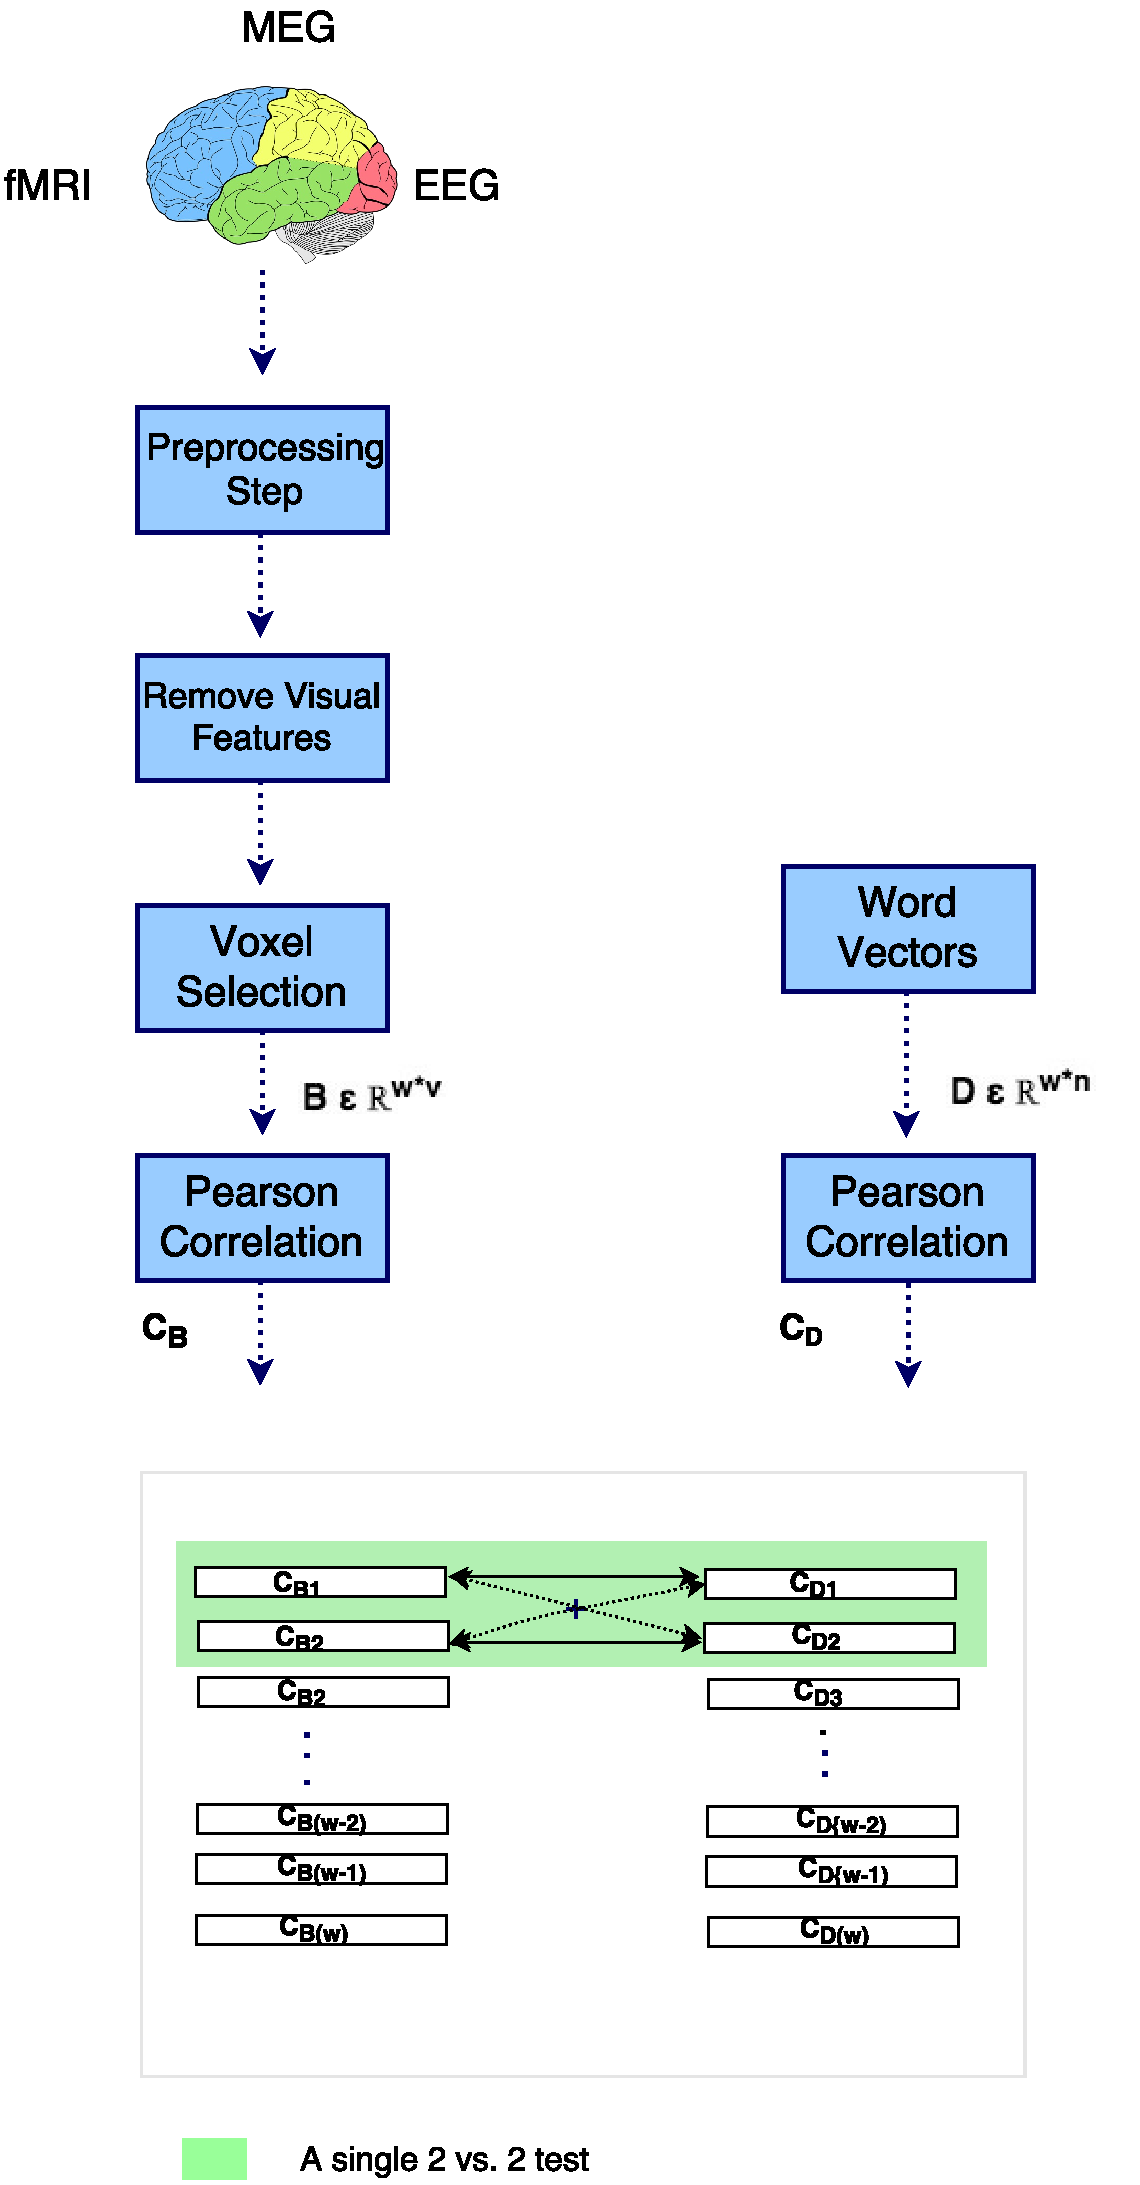
\includegraphics[width=10cm, height=20cm]{Figures/BrainBenchDiagram1}
\caption{The methodology for BrainBench test suite}
\label{BrainBenchMethod}
\end{figure}

\subsubsection{\underline{Removing Visual Features using Linear Regression}}

The visual features are removed by training a linear regression model which predicts a value per voxel corresponding to the visual features in the brain signal. These learned visual features are subtracted from the original brain signal. A linear regression model tries to fit a straight line for a set of data points in such a way that the sum of squared errors is minimal [Figure:~\ref{LinearRegression}].  We learn the weight matrix ($\mathbf w$) which parameterizes the best fit line for every data point $(\mathbf x_i, y_i)$. Let us define the error $e_i$ as the distance between the true and predicted values such that $e_i = y_i - \mathbf w^T \mathbf x_i$. The objective function of the linear regression model is to minimize the the sum of squared errors such that $\sum e_i^2 =  \| X \mathbf w - \mathbf y \|^2$, where ($\mathbf X$)  in our context are the visual features for each trial in our experiment and $\mathbf y$ is the brain signal. 



\begin{figure}[t]
\centering
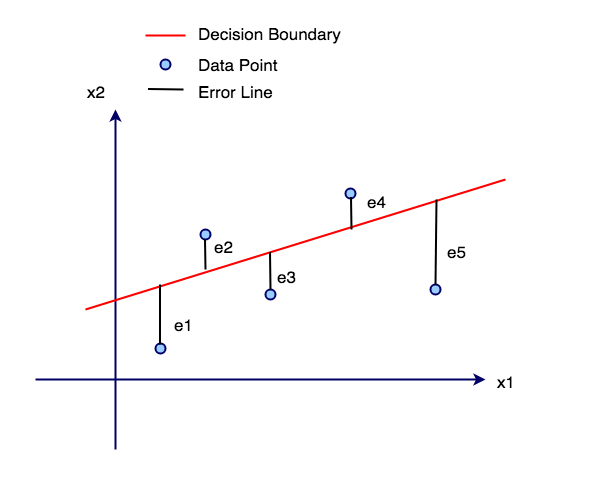
\includegraphics[width=10cm, height=8cm]{Figures/LinearRegression}
\caption{A concept diagram for Linear Regression}
\label{LinearRegression}
A Linear Regression model tries to fit a straight line for a set of data points in such a way that the sum of squared errors is minimal.
\end{figure}

Sometimes the visual features might be correlated with one another. An example could be the length of words could be correlated with the number of black pixels on the screens used to represent the word. This can result in the weight matrix ($\mathbf w$) being poorly determined and could result in over-fitting. This collinearity between visual features could cause the $\mathbf w$ to have substantial updates for a particular training sample and therefore may not generalize across all other samples in the data. Therefore, we introduce weight decay to restrict the updates to the weight matrix ($\mathbf w$) in the presence of very large values in the feature matrix ($\mathbf X$). This is also known regularization. The objective function of a linear regression model with regularization is given as %
\[\min\limits_{\mathbf w} \| X \mathbf w - y \|^2 + \lambda \, \| \mathbf w \|^2\]

Where $\lambda$ is a hyper-parameter. The regularization followed here is also knows as L2 regularization. The L2 regression performed here has a closed form solution. For each voxel in the brain signal, the regression model predicts a value as a function of the visual features, and this predicted value is then subtracted from the original voxel value.  This method is also termed as \textbf{``partialling out''} an effect. It should be noted that the only visual features removed from the Italian fMRI and EEG data were the length of words.
\subsubsection{\underline{Voxel Selection}}
The brain data after the removal of visual features still contains noise. We followed the same methodology used by Mitchell et al. \cite{Mitchell1191} to select the most stable voxels. In this process, we choose only those voxels which show strong self-correlation across various trials of the same word. The voxels which have such strong self-correlations would have a high stability score. Here, we assume that any voxel with a low stability score could be noise and is not considered for our experiments. Roughly, around 500 voxels from each dataset were selected and used in our study.

\subsubsection{\underline{Pearson Correlation}}
The brain data corresponding to repetitions of the same word are then averaged for each participant resulting in a matrix $\ B\in \mathbb{R} ^{w*v}$, where $w$ is the number of words, and $v$ is the number of voxels selected. We then calculate the Pearson correlation of every row in brain data $\ B$ with every other row resulting in the brain correlation matrix ($C_B$) where $\ C_B\in \mathbb{R} ^{w*w}$. Each row $C_{B_i}$ of the matrix $C_B$ represents the correlation of the word $i$ with every other word from $1$ to $w$ in the brain imaging dataset.

The same approach is followed for the DS models. From each DS model, we extract the words that are present in the model and the brain datasets resulting in the matrix $\ D\in \mathbb{R} ^{w*n}$, where $w$ is the number of words and n is the number of dimensions of the word vector. We then compute the Pearson correlation of every word in word vector matrix $D$ with every other word in the matrix resulting in the correlation matrix $C_D$ where $\ C_D\in \mathbb{R} ^{w*w} $.


\newpage
\textbf{The similarity between $C_B$ and $C_D$ could be studied using the 2 vs. 2 test which is described below.}

\begin{figure}[!b]
\centering
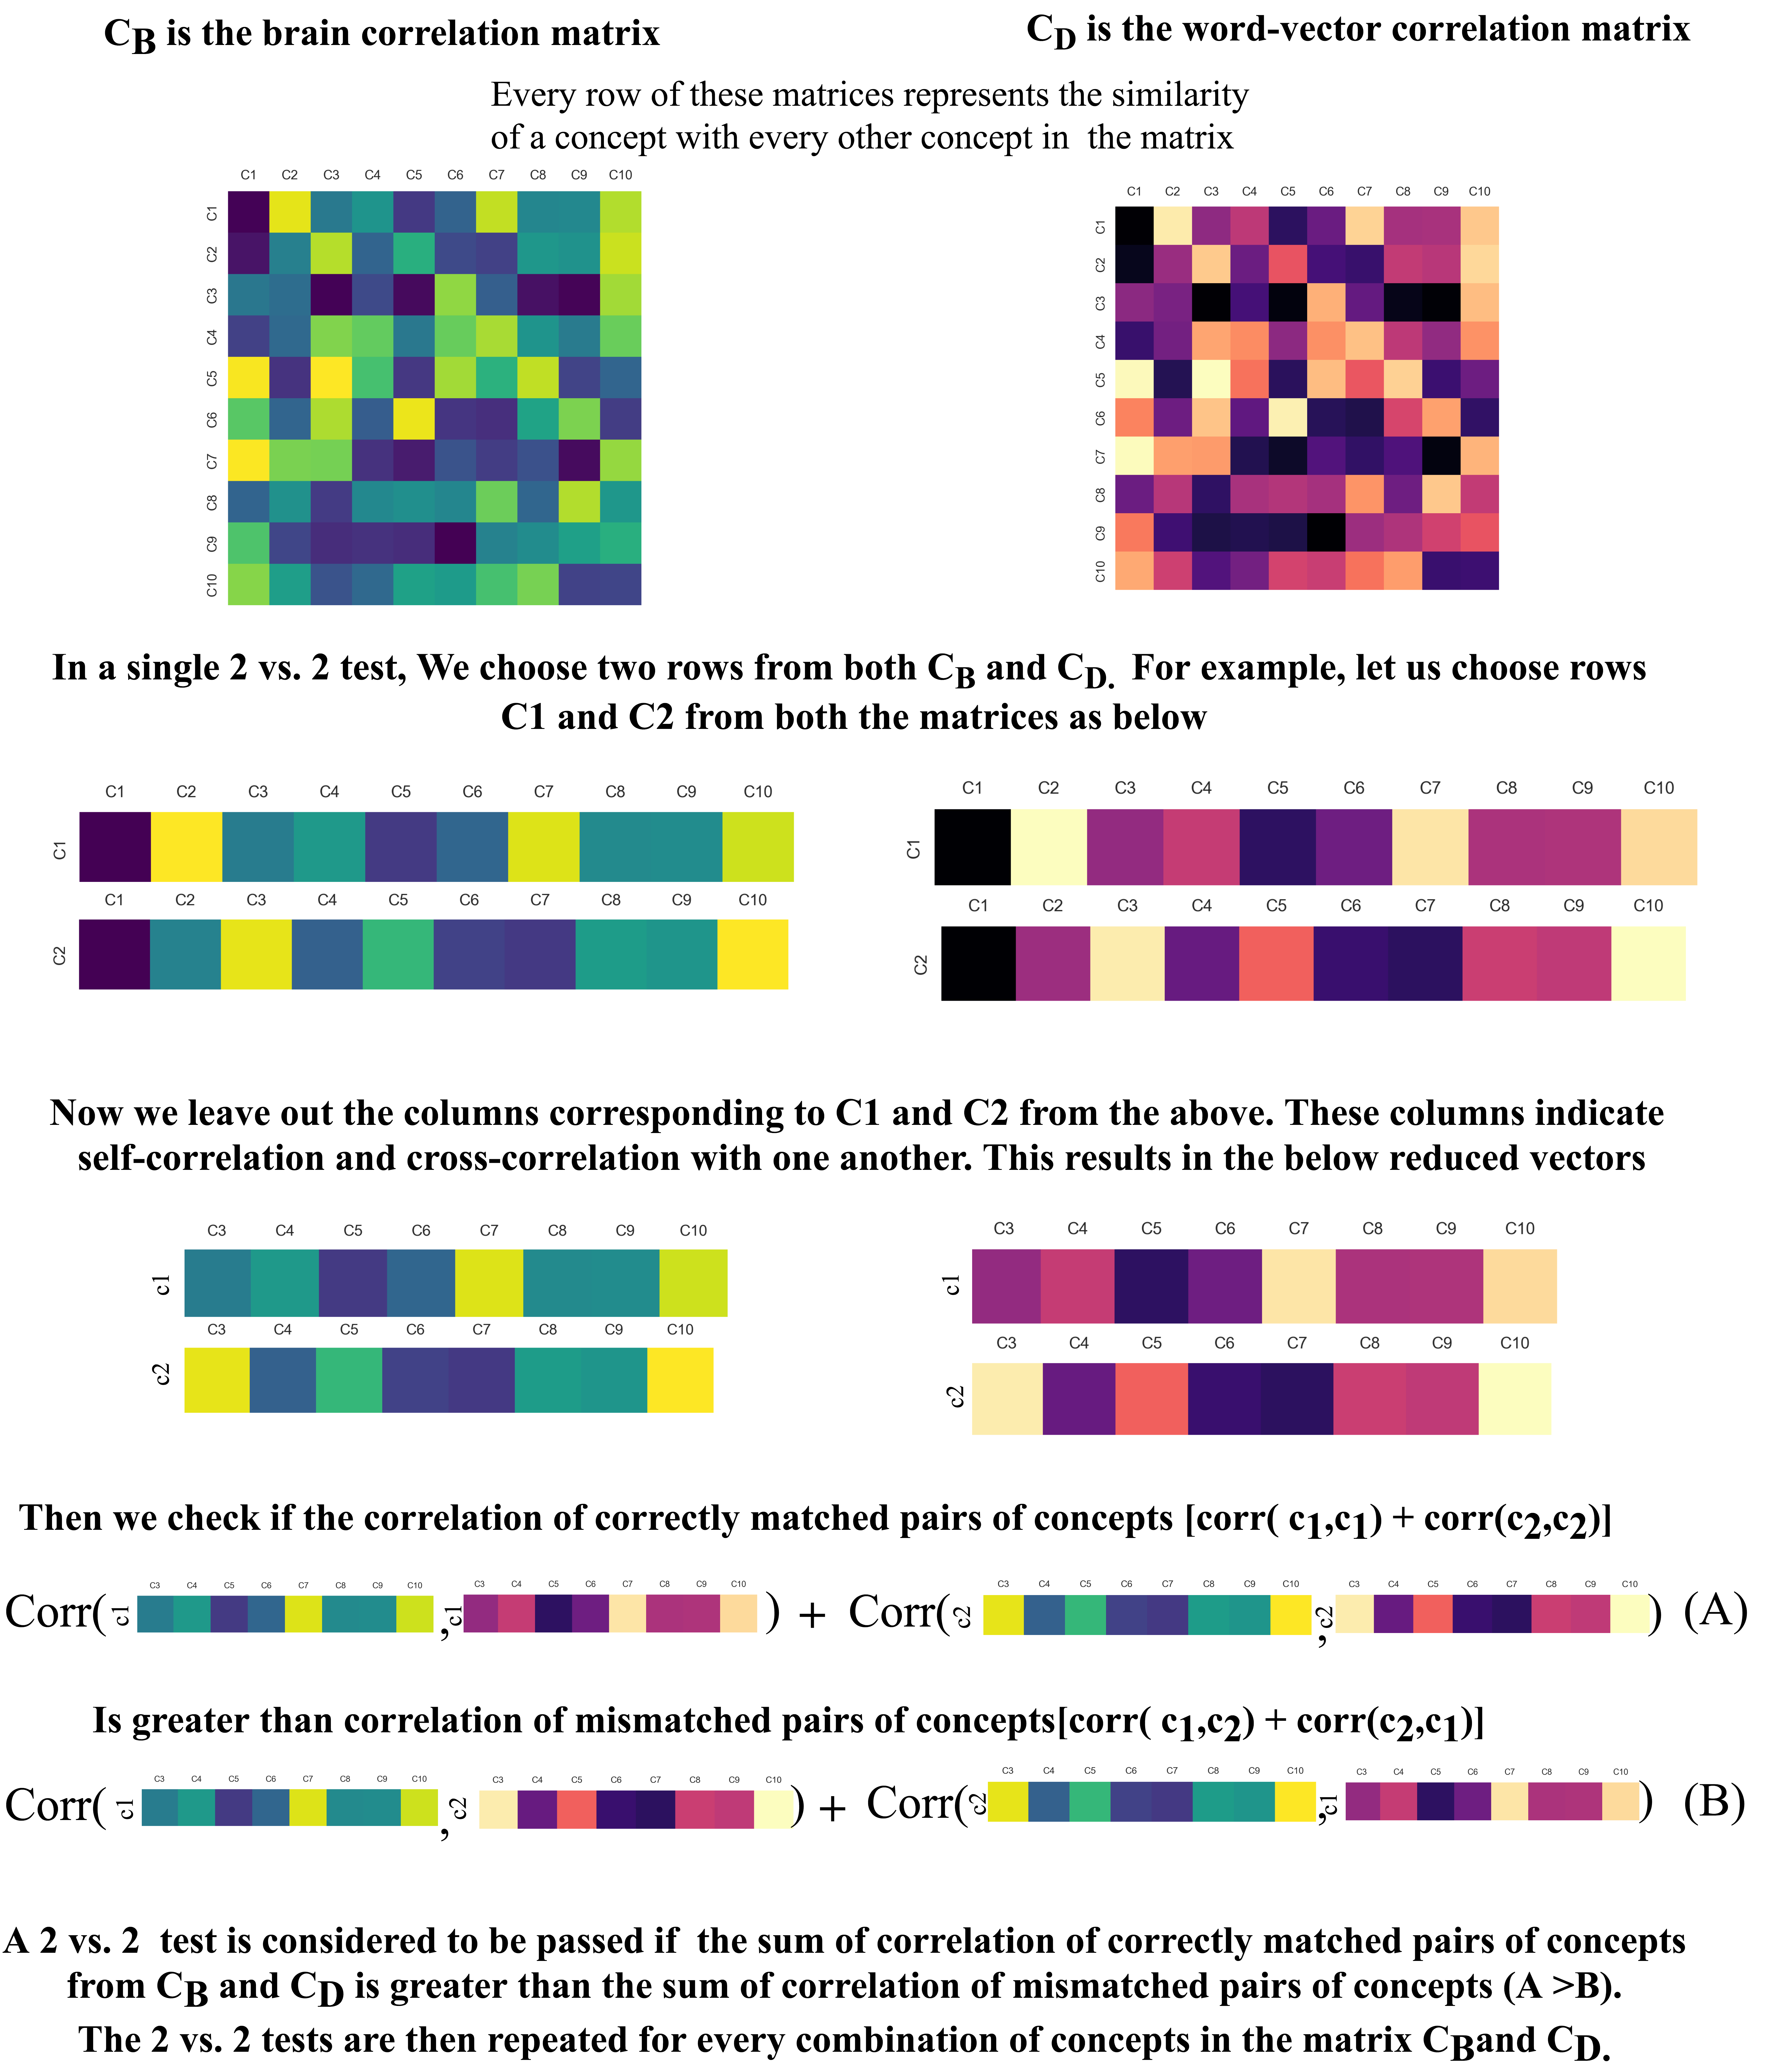
\includegraphics[width=14cm, height=18cm]{Figures/2vs2brainbench}
\caption{A Pictorial Representation of 2 vs. 2 test.}
\label{2vs2bb}
This figure depicts an example of the 2 vs. 2 test demonstrated for 10 concepts.
\end{figure}
\newpage

Now we have created two correlation matrices $C_B$ and  $C_D$ representing similarity of words in different vector spaces. We could use the Representational Similarity Analysis (RSA) method to compute the correlation between matrices $C_B$ and  $C_D$ \cite{RSA}. RSA is a simple method adopted from the field of neuroscience to study the relationship between two vector spaces. However, the RSA has a disadvantage that it produces one aggregate score for the relationship between two matrices. As we will see, it is sometimes essential to study and understand the parts of the correlation matrix which may result in a high or low score. 


\subsubsection{\underline{2 vs. 2 Tests}}
Instead of measuring the correlation between the matrices $C_B$ and  $C_D$ using RSA, we perform the 2 vs. 2 test derived from the early works of Mitchell et al. searching for word embeddings in the brain \cite{Mitchell1191}. This methodology introduced by  Anderson et al. \cite{Andrew2vs2} and Xu et al. \cite{BrainBench2016} could be considered as an extension of RSA with the 2 vs. 2 test. In 2 vs. 2, we select the rows corresponding to two concepts ($c_1$ and $c_2$) from our correlation matrices $C_B$ and  $C_D$. We then omit the columns corresponding to two concepts resulting in a reduced vector with $w-2$ columns from both the matrices where $w$ is the total number of concepts. These vectors represent the similarity of the two concepts with every other concept, except for their self correlation and their correlation with one another. Let us call the reduced vectors as
$C_{B_1}$, $C_{B_2}$ from correlation matrix $C_B$ and $C_{D_1}$, $C_{D_2}$ from correlation matrix $C_D$. The correlation of the concepts $c_1$ and $c_2$ from $C_B$ and  $C_D$  are then computed to check if the correlation of the correctly matched pairs:

\[corr(C_{B_1},C_{D_1}) + corr(C_{B_2},C_{D_2})  \]

\noindent is greater than the correlation of the mismatched pairs:

\[corr(C_{B_1},C_{D_2}) + corr(C_{B_2},C_{D_1})  \]

A 2 vs. 2 test is considered to be passed if the correlation of the matched pairs is greater than the correlation of the mismatched pairs. The test is repeated for all possible pairs of concepts in our dataset. This results in $^wChoose_2$ tests for a dataset, where $w$ is the number of rows in the correlation matrix. The 2 vs. 2 accuracies is the percentage of the number of 2 vs. 2 tests passed to the total number of 2 vs. 2 tests. since this is a binary classification task, the chance accuracy is 50\%. A pictorial representation of the test is described by Figure:~\ref{2vs2bb}.


The methodology described in this section (Figure:~\ref{BrainBenchMethod}) varies from the method described by Xu et al.~\cite{BrainBench2016}.  We remove visual features before voxel selection as compared to the Xu et al. where voxel selection was performed before removing visual features from the brain signal.  We believe that, if voxel selection is performed without removing visual features from the signal, the most stable voxels selected could be the ones which are correlated with visual features rather than semantics.


\subsubsection{Statistical Significance Tests}

The 2 vs. 2 test was designed to study and compare the relationship between concepts in different vector spaces. The chance accuracy is 50\%. In statistics, a null hypothesis is a hypothesis that there exists no relationship between the variables that we are trying to compare. In our tests, the null hypothesis is that there is no similarity between correlation concepts in brain data and word-vector space. Let us define the level of significance ($\alpha$) as the probability of rejecting the null hypothesis and p-value ($p$) as the probability of our tests returning extreme values, both assuming that the null hypothesis is true. Therefore, for us to reject the null hypothesis and to prove concretely that our results are statistically significant, we look for $p < \alpha$

We conduct 1000 permutation tests by randomly shuffling the assignment of word identity to word-vector, recomputing the $C_D$, and re-running the 2 vs. 2 tests for each permutation. After the permutation tests, the p-value is calculated as 

\[p = R/T\] where R is the number of random permutation accuracies which is greater than or equal to the observed accuracy of our tests and T is the number of random permutations conducted. For example, if the 2 vs. 2 accuracy is 0.63 and 1000 random permutations tests returned 14 2 vs. 2 accuracy values greater than our observed accuracy, then the p-value for this experiment is 0.014 (R=14 and T=1000). The statistical significance depends heavily on the level of significance ($\alpha$) which is usually fixed at 5\%. In our example here $p < \alpha$ (0.014 $<$ 0.050) and therefore, we can reject the null hypothesis that there is no correlation between the two vector spaces.
\section{Evaluation of DS models against anatomical brain region}

Anderson et al.,2015 performed exploratory analysis studying the correlation of both image and corpora based features with various Regions of Interest (ROI) in human brain~\cite{Anderson2015}. They also provided evidence that for a given concept, text-based DS models showed similarity in fMRI scans in ROI's related to linguistic processing. Similarly, image-based models showed similarity with ROI related to visual processing in the human brain. We incorporate into BrainBench the ability to evaluate DS models against various ROI in human brain using the same fMRI data collected by Mitchell et al., 2008~\cite{Mitchell1191}


The size and shape of brain vary across different individuals. It, therefore, becomes essential to spatially normalize fMRI data from various participants in the study such that a location in one person's brains scan corresponds to the same location in other persons brain scan. The fMRI data after pre-processing was spatially normalized into Montreal Neurological Institute space (MNI) and resampled to 3mm x 3mmx 6mm voxels. MNI is a  template which divides the brain into various regions of interest. Each voxel in the fMRI data is associated with a spatial position involving 3D coordinates ($x,y,z$) in the human brain. The voxel coordinates could be converted into MNI coordinates using the SPM software in Matlab to map a single voxel to an ROI in the brain.

After regressing out the visual features from the brain data, we extracted the voxels corresponding to various ROIs in the brain for each of 60 concepts. This results in $60*v$ matrix for every anatomical region that we were included in our experiments. Here $v$ is again the number of voxels. We ignore regions with $v < 200$ in our fMRI data across all 9 participants. It should also be noted that voxel selections were not performed as a part of this study since the number of available voxels per region was limited. The experiments then followed the process explained under the section \ref{brainbenchmethod}. The 2 vs. 2 tests were conducted for every anatomical ROIs in the brain which satisfied the condition of a minimum of 200 voxels in all 9 participants. Statistical significance tests were run for all combinations of ROIs and DS models.
\section{Results and Discussions}

\begin{figure}[!t]
\centering
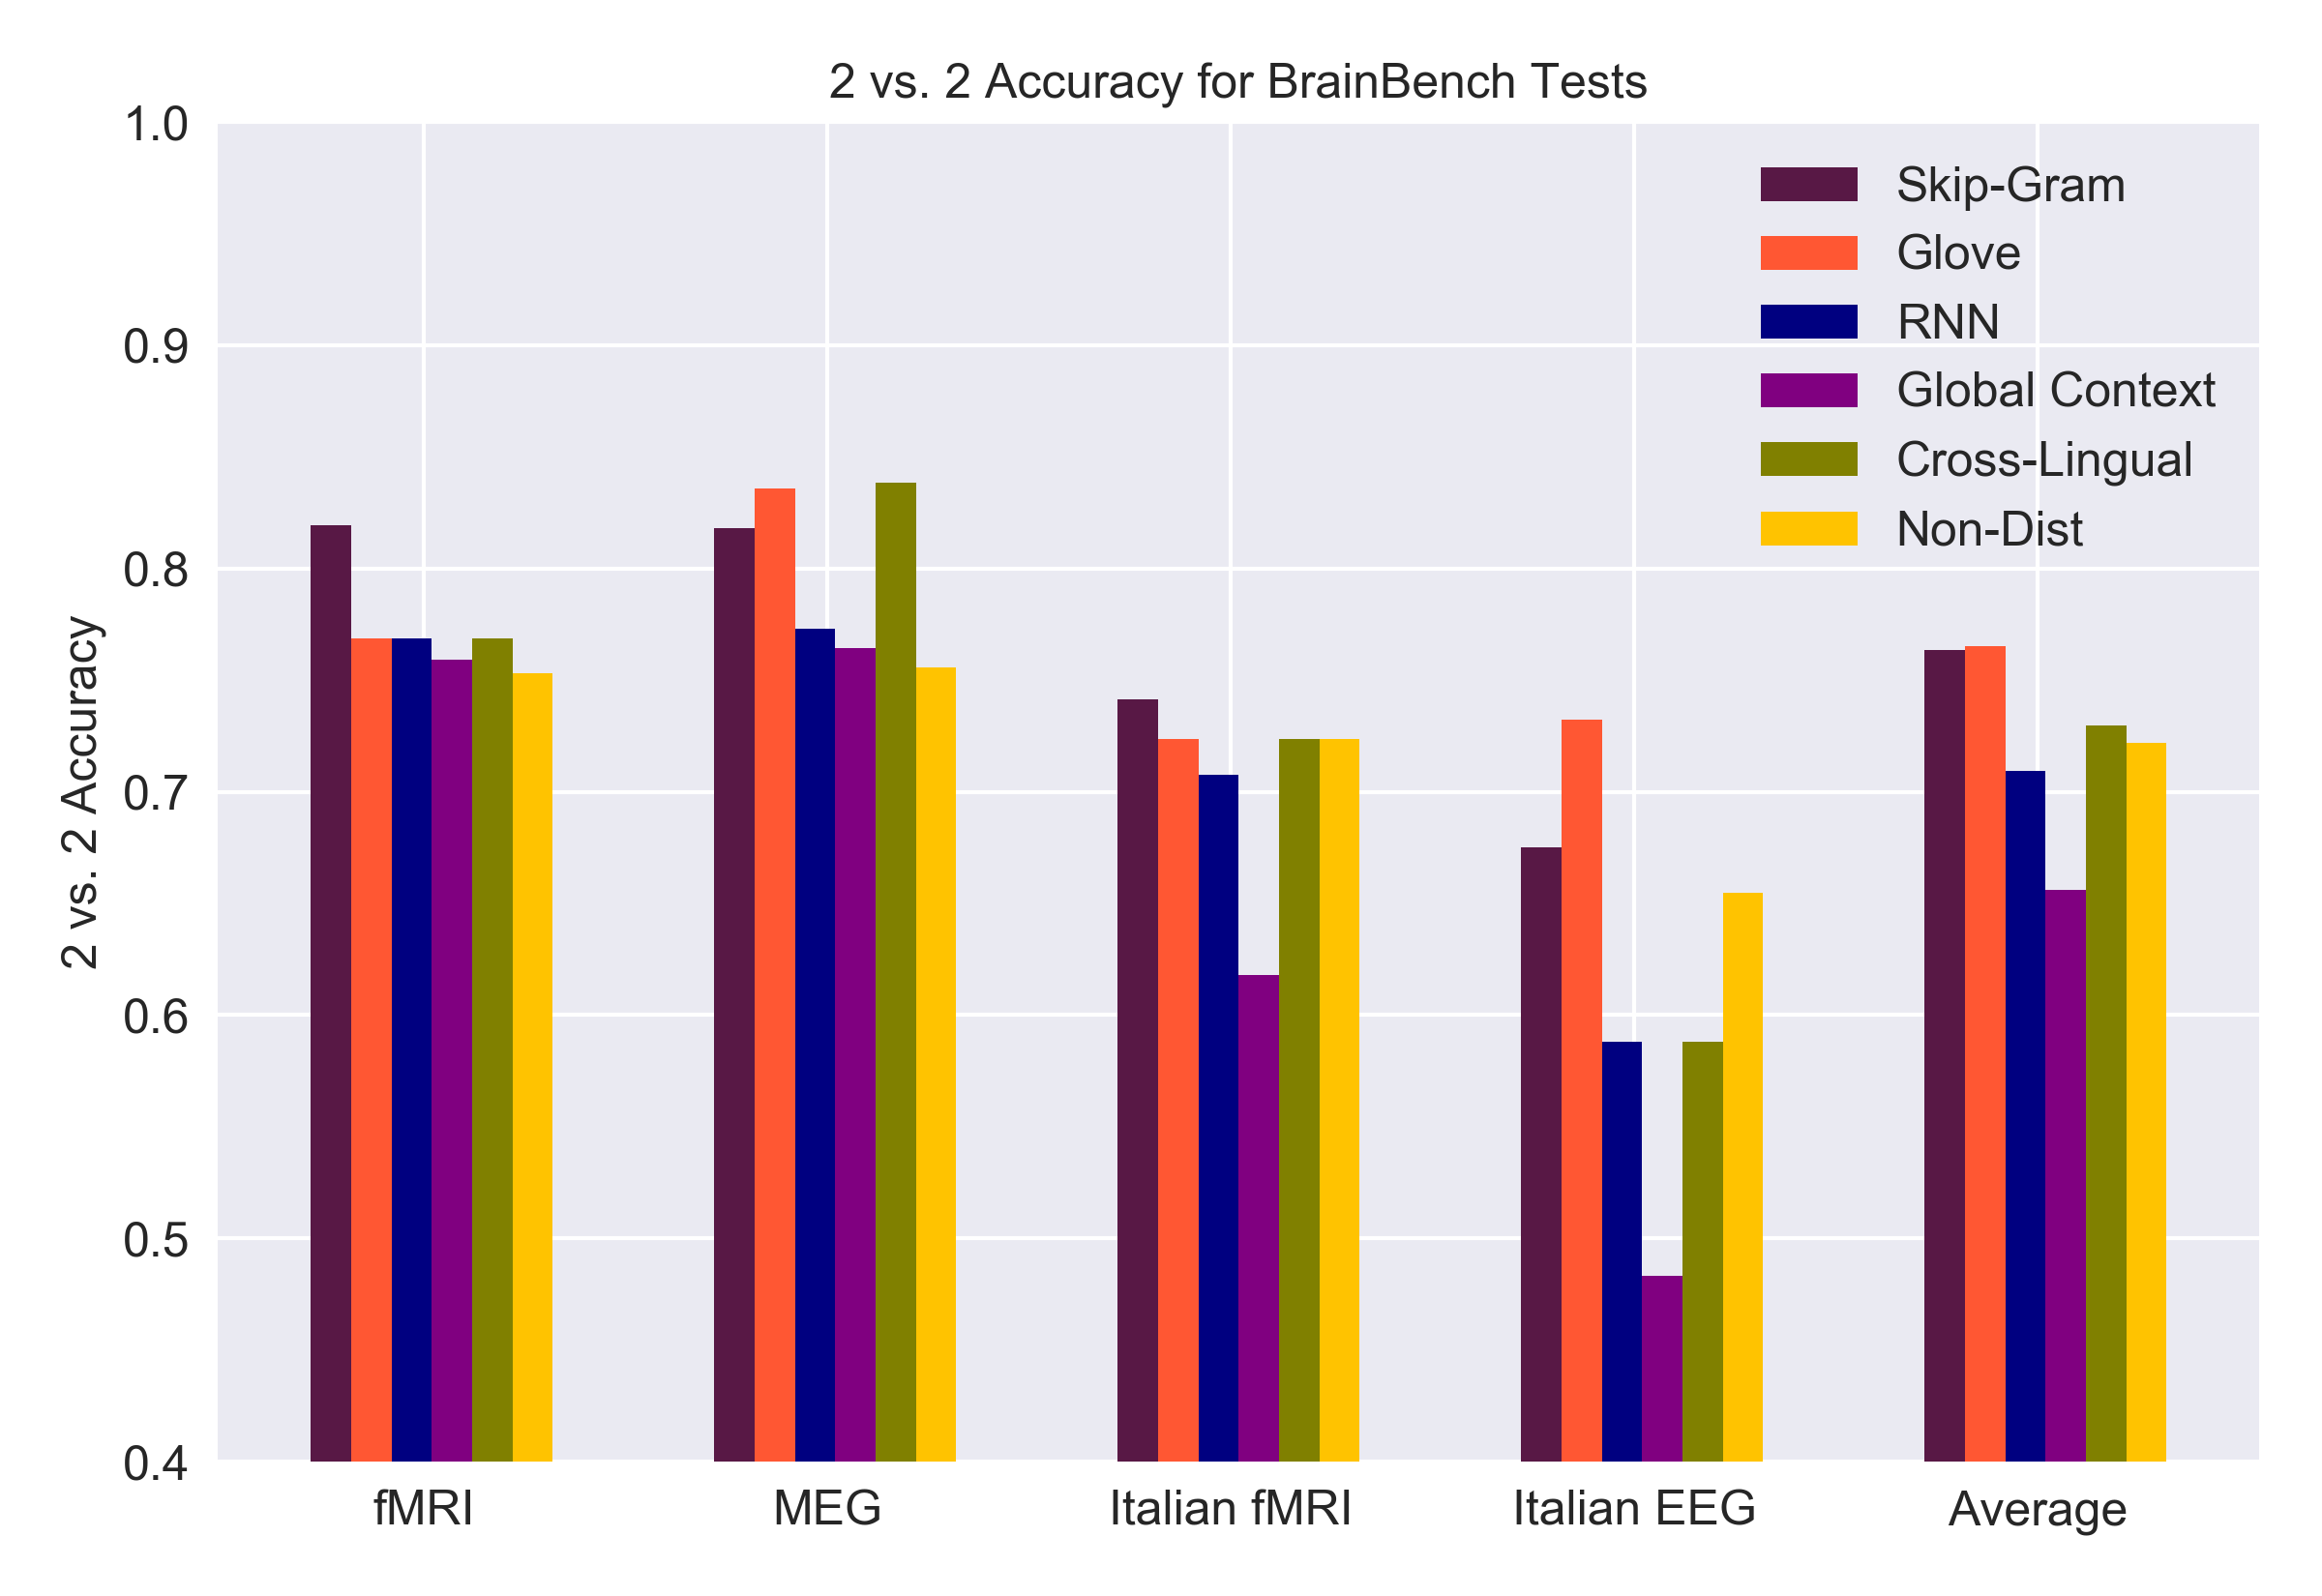
\includegraphics[width=14cm, height=9cm]{Figures/BrainBenchSummary1}
\caption{Summary of BrainBench Test Results}
\label{BrainBenchSummary}
The fMRI and MEG contains 60 concrete concepts, Italian fMRI contains 70 concepts from two domains, and 7 taxonomic categories with varying degree of concreteness, and finally, the Italian EEG contains 30 concrete concepts from each Mammals, and Tools category.
\end{figure}
In this section, we report the results of our experiments involving the evaluation of 6 popular word vector models against 4 different brain datasets using the 2 vs. 2 tests. These results are summarized in Figure:~\ref{BrainBenchSummary}.  The permutations tests were run for all possible pairs of brain datasets and DS models. Except for the 2 vs. 2 accuracy for the Global-Context with the Italian EEG dataset, all other 2 vs. 2 accuracies were found to be statistically significant with $p<0.01$.

There is a significant variance in the performance of different word vectors on different brain datasets. Skip-Gram and Glove are the best performing DS models across all the 4 datasets whereas Global-Context performs the worst. The Global-Context vectors have the smallest number of dimensions (50) as compared to other word vectors like Skip-gram (300), Glove (300), RNN (640), Cross-Lingual (512) etc. Prior Research by Mikolov et al., 2013 have shown that there is a positive correlation between the number of vector dimensions in a word vector and their corresponding performance on various downstream NLP tasks~\cite{Word2Vec}. They found that for the Skip-gram model, vectors with dimensions around 300 were most suited for downstream NLP tasks compared to Skip-gram models with 50 dimensions or less. 





Global-Context vectors may not also be encoding enough semantic information due to the smaller size of its vectors. Moreover, Global-Context vectors were also shown to perform poorly on other word similarity datasets (Figure:~\ref{wordsimcomparison}) which is consistent with the results of BrainBench tests.

The fMRI and MEG dataset in BrainBench has higher accuracies compared to both Italian fMRI and EEG (Figure:~\ref{BrainBenchSummary}). It should also be noted that performance of Glove is comparatively better in both MEG and EEG dataset. Prior research has shown that word vectors based on word co-occurrences do capture temporal dynamics of semantics~\cite{TemporalDynamics}. EEG and MEG also incorporate temporal information from the brain signal, and therefore one could speculate that Glove vectors could also be incorporating higher temporal dynamic related to semantics compared to all other word vectors. 


\subsection{Concrete Vs Abstract Nouns}
The 2 vs. 2 accuracy for Italian fMRI scores are slightly lower (8-10\% for various DS models) compared to the English language based fMRI. It should be noted that the Italian fMRI has a larger distribution of abstract words as compared to English fMRI (only concrete nouns). Anderson et al., 2015 studying the \textit{varying degree of concreteness} through their experiments on the same Italian dataset have shown that decoding semantics from neural signals corresponding abstract nouns are more difficult as compared to concrete nouns~\cite{AndersonConcreteness}. We also attribute our lower 2 vs. 2 accuracy for the Italian fMRI due to the higher distribution of abstract nouns in the dataset.
\begin{figure}[!hb]
\centering
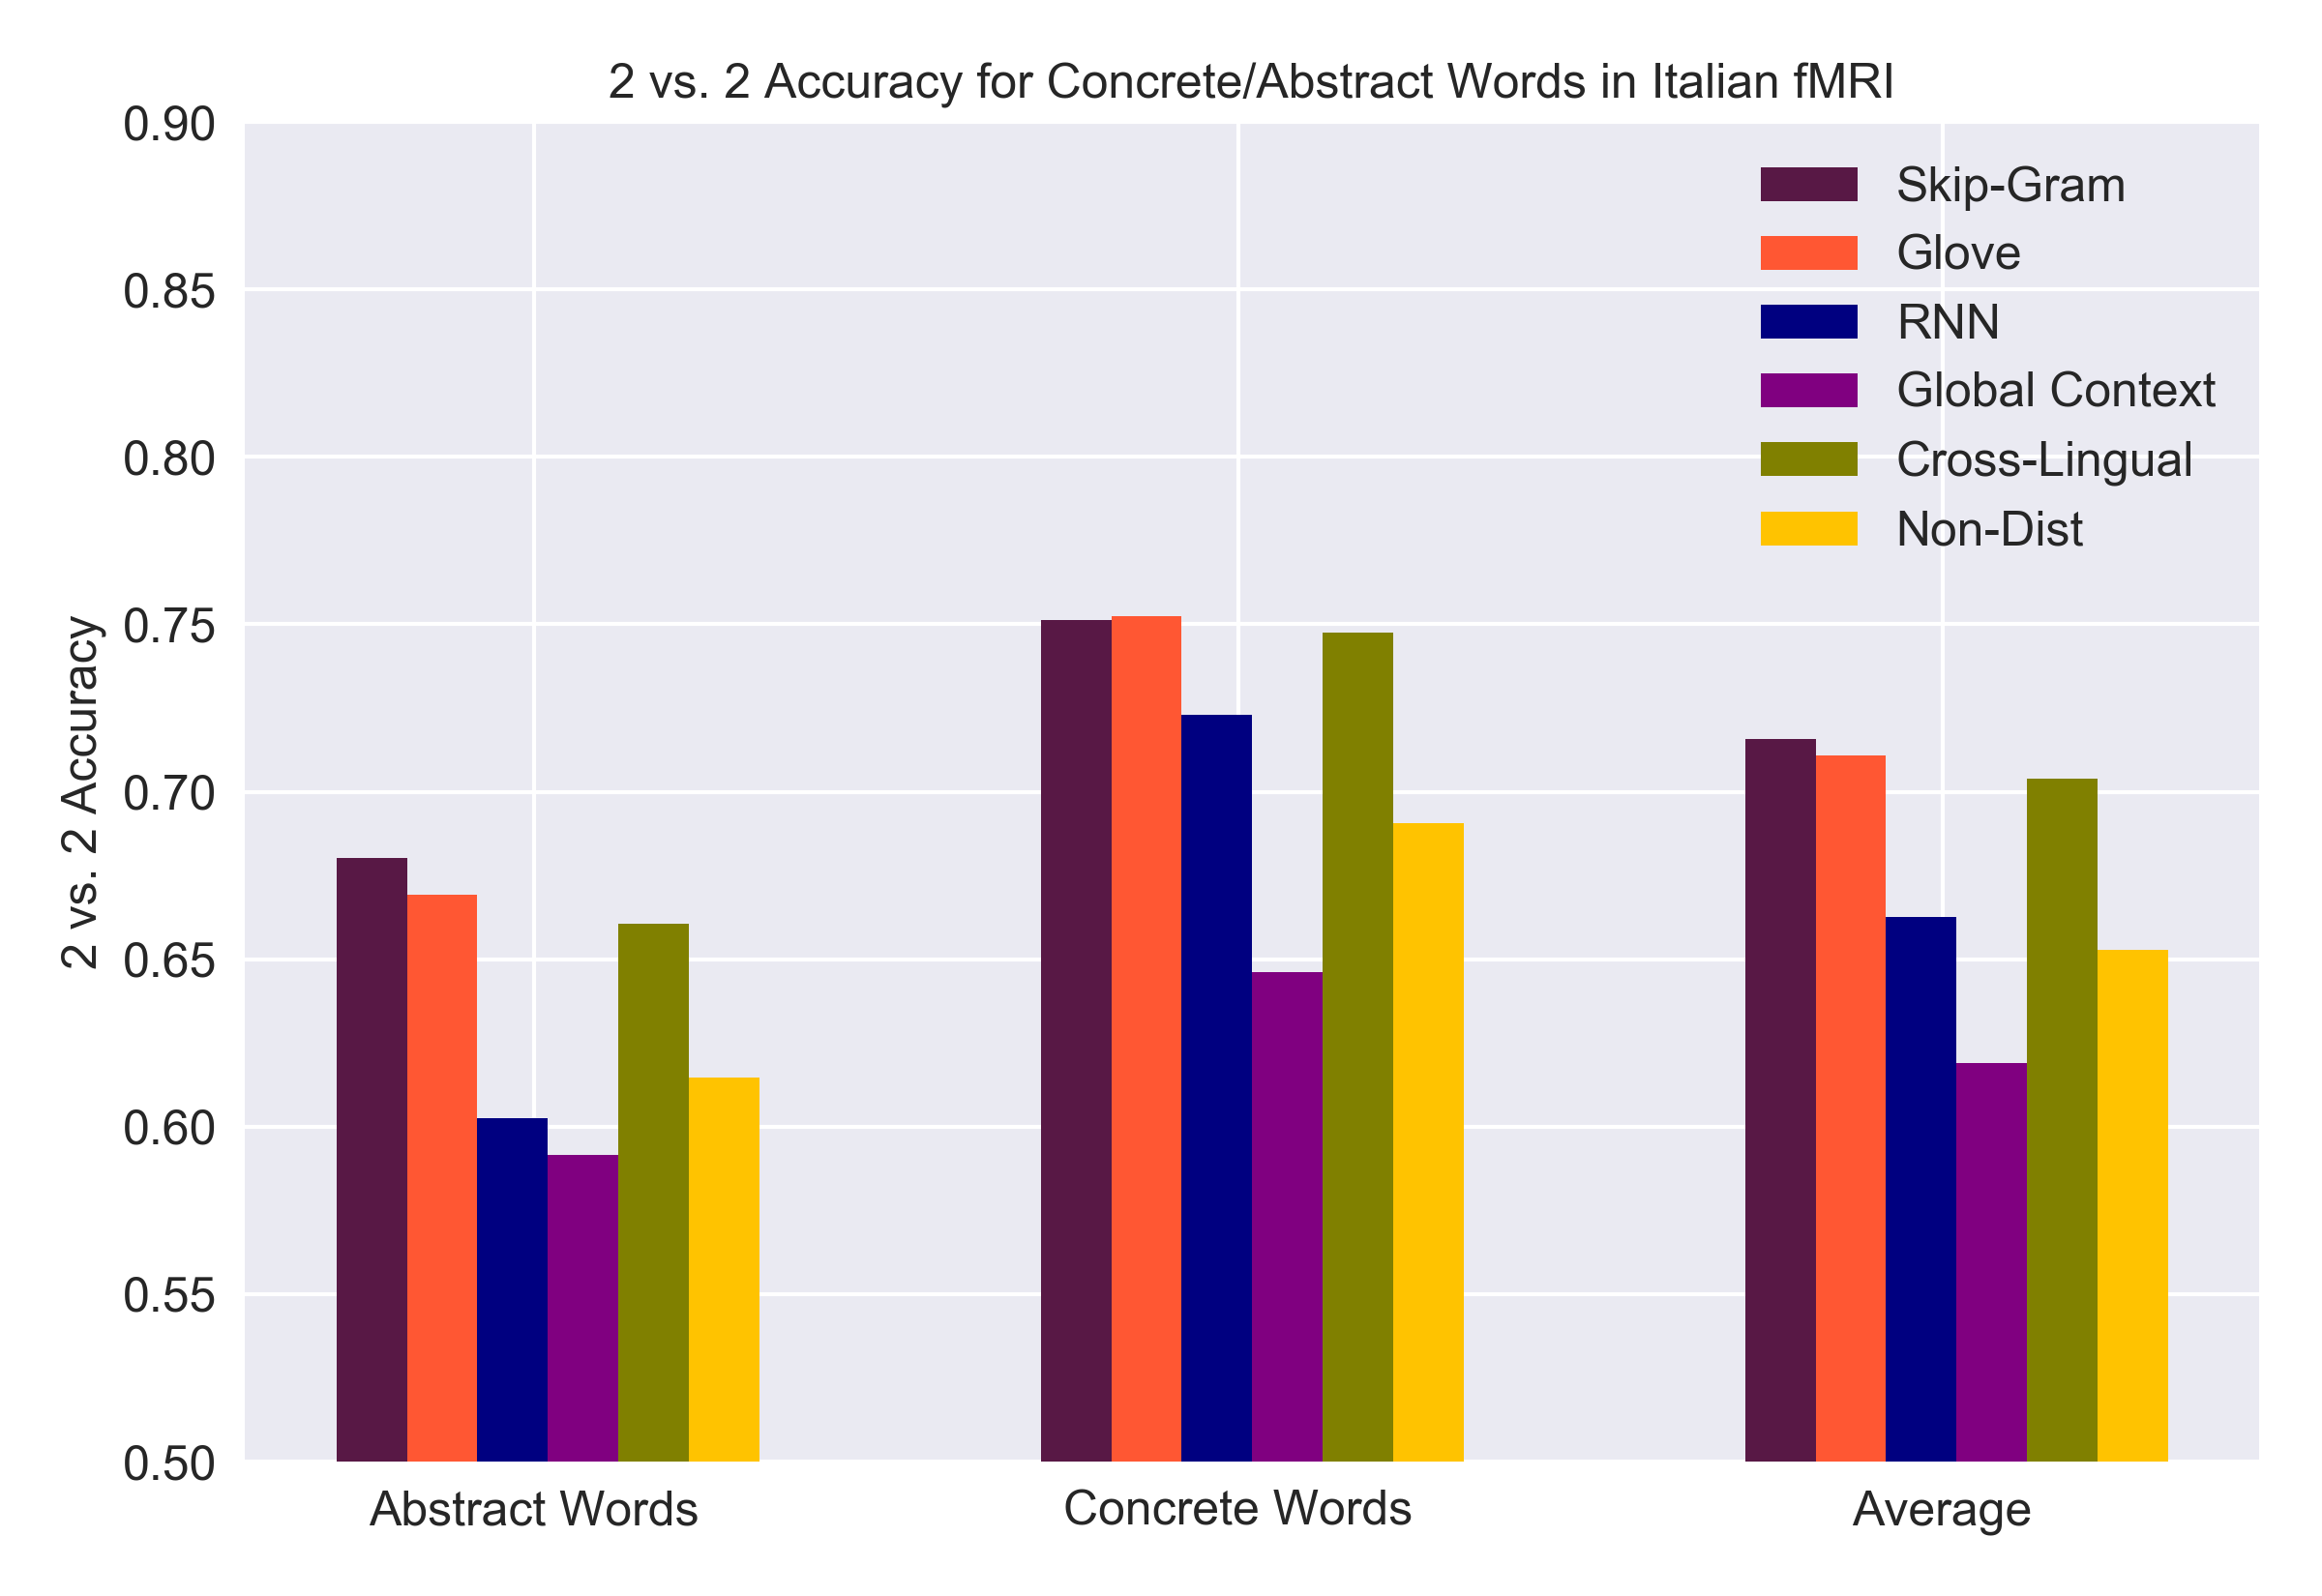
\includegraphics[width=14cm, height=9cm]{Figures/Italian}
\caption{Concrete Vs Abstract scores for Italian fMRI}
\label{ItalianSummary}
\end{figure}
We performed a comparative study of the 2 vs. 2 accuracy for concrete and abstract nouns separately in the Italian fMRI. We selected words from three taxonomic categories (Tool, Location and Social Role) as concrete and other four taxonomic categories (Event, Communication, Attribute, Urabstracts) as abstract based on the Figure:~\ref{ItalianFMRI}. This figure represents the taxonomic categories on a binarized concreteness scale with concrete being 1 and abstract being 0. The three taxonomic categories (Tool, Location and Social Role) in the figure are more shifted towards being concrete as compared to other four taxonomic categories. Thus the dataset was divided into 30 concrete and 40 abstract words.

The 2 vs. 2 accuracies for abstract words were at least $10\%$ to $12\%$ lower than the 2 vs. 2 accuracies for concrete words in the datasets. These results are again consistent with the ones reported by Anderson et al., 2015~\cite{AndersonConcreteness}. Moreover, unlike concrete nouns, \textit{``an individuals experience of abstract nouns may be subjective''} and could vary from person to person~\cite{AndersonConcreteness}. It is also highly unlikely that the corpus-based language models could capture the large variability in the abstract nouns representations arising from subjectivity based on human experience. The performance of various DS models on Italian fMRI dataset is summarized by the Figure:~\ref{ItalianSummary}.

%Talk about EEG dataset and Coverage.

\begin{table}[t]
\centering

\begin{tabular}{|c|c|c|c|c|c|c|c|}
\hline
\textbf{\begin{tabular}[c]{@{}c@{}}Brain \\ Datasets\end{tabular}} & \textbf{\begin{tabular}[c]{@{}c@{}}Total \\concepts\end{tabular}} & \textbf{\begin{tabular}[c]{@{}c@{}}Skip-\\ Gram\end{tabular}} & \textbf{Glove} & \textbf{RNN} & \textbf{\begin{tabular}[c]{@{}c@{}}Global \\ Context\end{tabular}} & \textbf{\begin{tabular}[c]{@{}c@{}}Cross-\\ Lingual\end{tabular}} & \textbf{\begin{tabular}[c]{@{}c@{}}Non-\\ Dist\end{tabular}} \\ \hline
fMRI                                                               & 60                                                                        & 60                                                            & 60             & 60           & 60                                                                 & 60                                                                & 60                \\ \hline
MEG                                                                & 60                                                                        & 60                                                            & 60             & 60           & 60                                                                 & 60                                                                & 60                \\ \hline
Italian fMRI                                                       & 70                                                                        & 66                                                            & 66             & 62           & 65                                                                 & 66                                                                & 66                \\ \hline
Italian EEG                                                        & 60                                                                        & 43                                                            & 43             & 42           & 43                                                                 & 44                                                                & 43                \\ \hline
\end{tabular}
\caption{Concept coverage in various DS models}
\label{ConceptCoverage}
\end{table}
\subsection{Evaluation of DS models against EEG datasets }
EEG datasets are generally considered to be noisy and have poor signal to noise ratio (SNR). The 2 vs. 2 accuracies for various DS models against the Italian EEG dataset is summarized in the Figure:~\ref{BrainBenchSummary}. Except for Glove word vector all other DS models are having their lowest accuracies against the EEG data as compared to both the fMRI's and MEG data. In fact, 2 vs. 2 accuracy of Global-Context vectors are below the chance accuracy of 50\% and did not pass the permutation tests. EEG dataset also had the lowest coverage of concepts in DS models as compared to other brain datasets in BrainBench (Check Table:~\ref{ConceptCoverage}). If a concept is not found in a DS model, the 2 vs.2 tests corresponding to that particular concept is omitted. 

Despite the lower 2 vs. 2 accuracies, the performance of BrainBench using the EEG dataset is comparable to another other word similarity datasets. EEG data is much cheaper and convenient to collect as compared to fMRI and MEG. Our results with the EEG dataset should encourage the scientific community to built larger EEG based brain test suites to evaluate and benchmark word vectors.

% Talk about Italian Skip-Gram
\subsection{2 vs. 2 test results for Italian Skip-gram}
We also download the Italian Skip-gram vectors and conducted the 2 vs. 2 tests against the Italian fMRI. The 2 vs. 2 test accuracy for this particular experiment was found to be 74.1\% which is quite similar to the accuracy with English language version of the Skip-gram vector. This result could imply that the BrainBench tests could generalize for testing word vectors modeled from different languages irrespective of the native language of individuals from whom the original brain data were collected.


%Comparisons with other Similarity datasets.
\subsection{Comparing BrainBench with other word similarity datasets}


\begin{figure}[t]
\centering
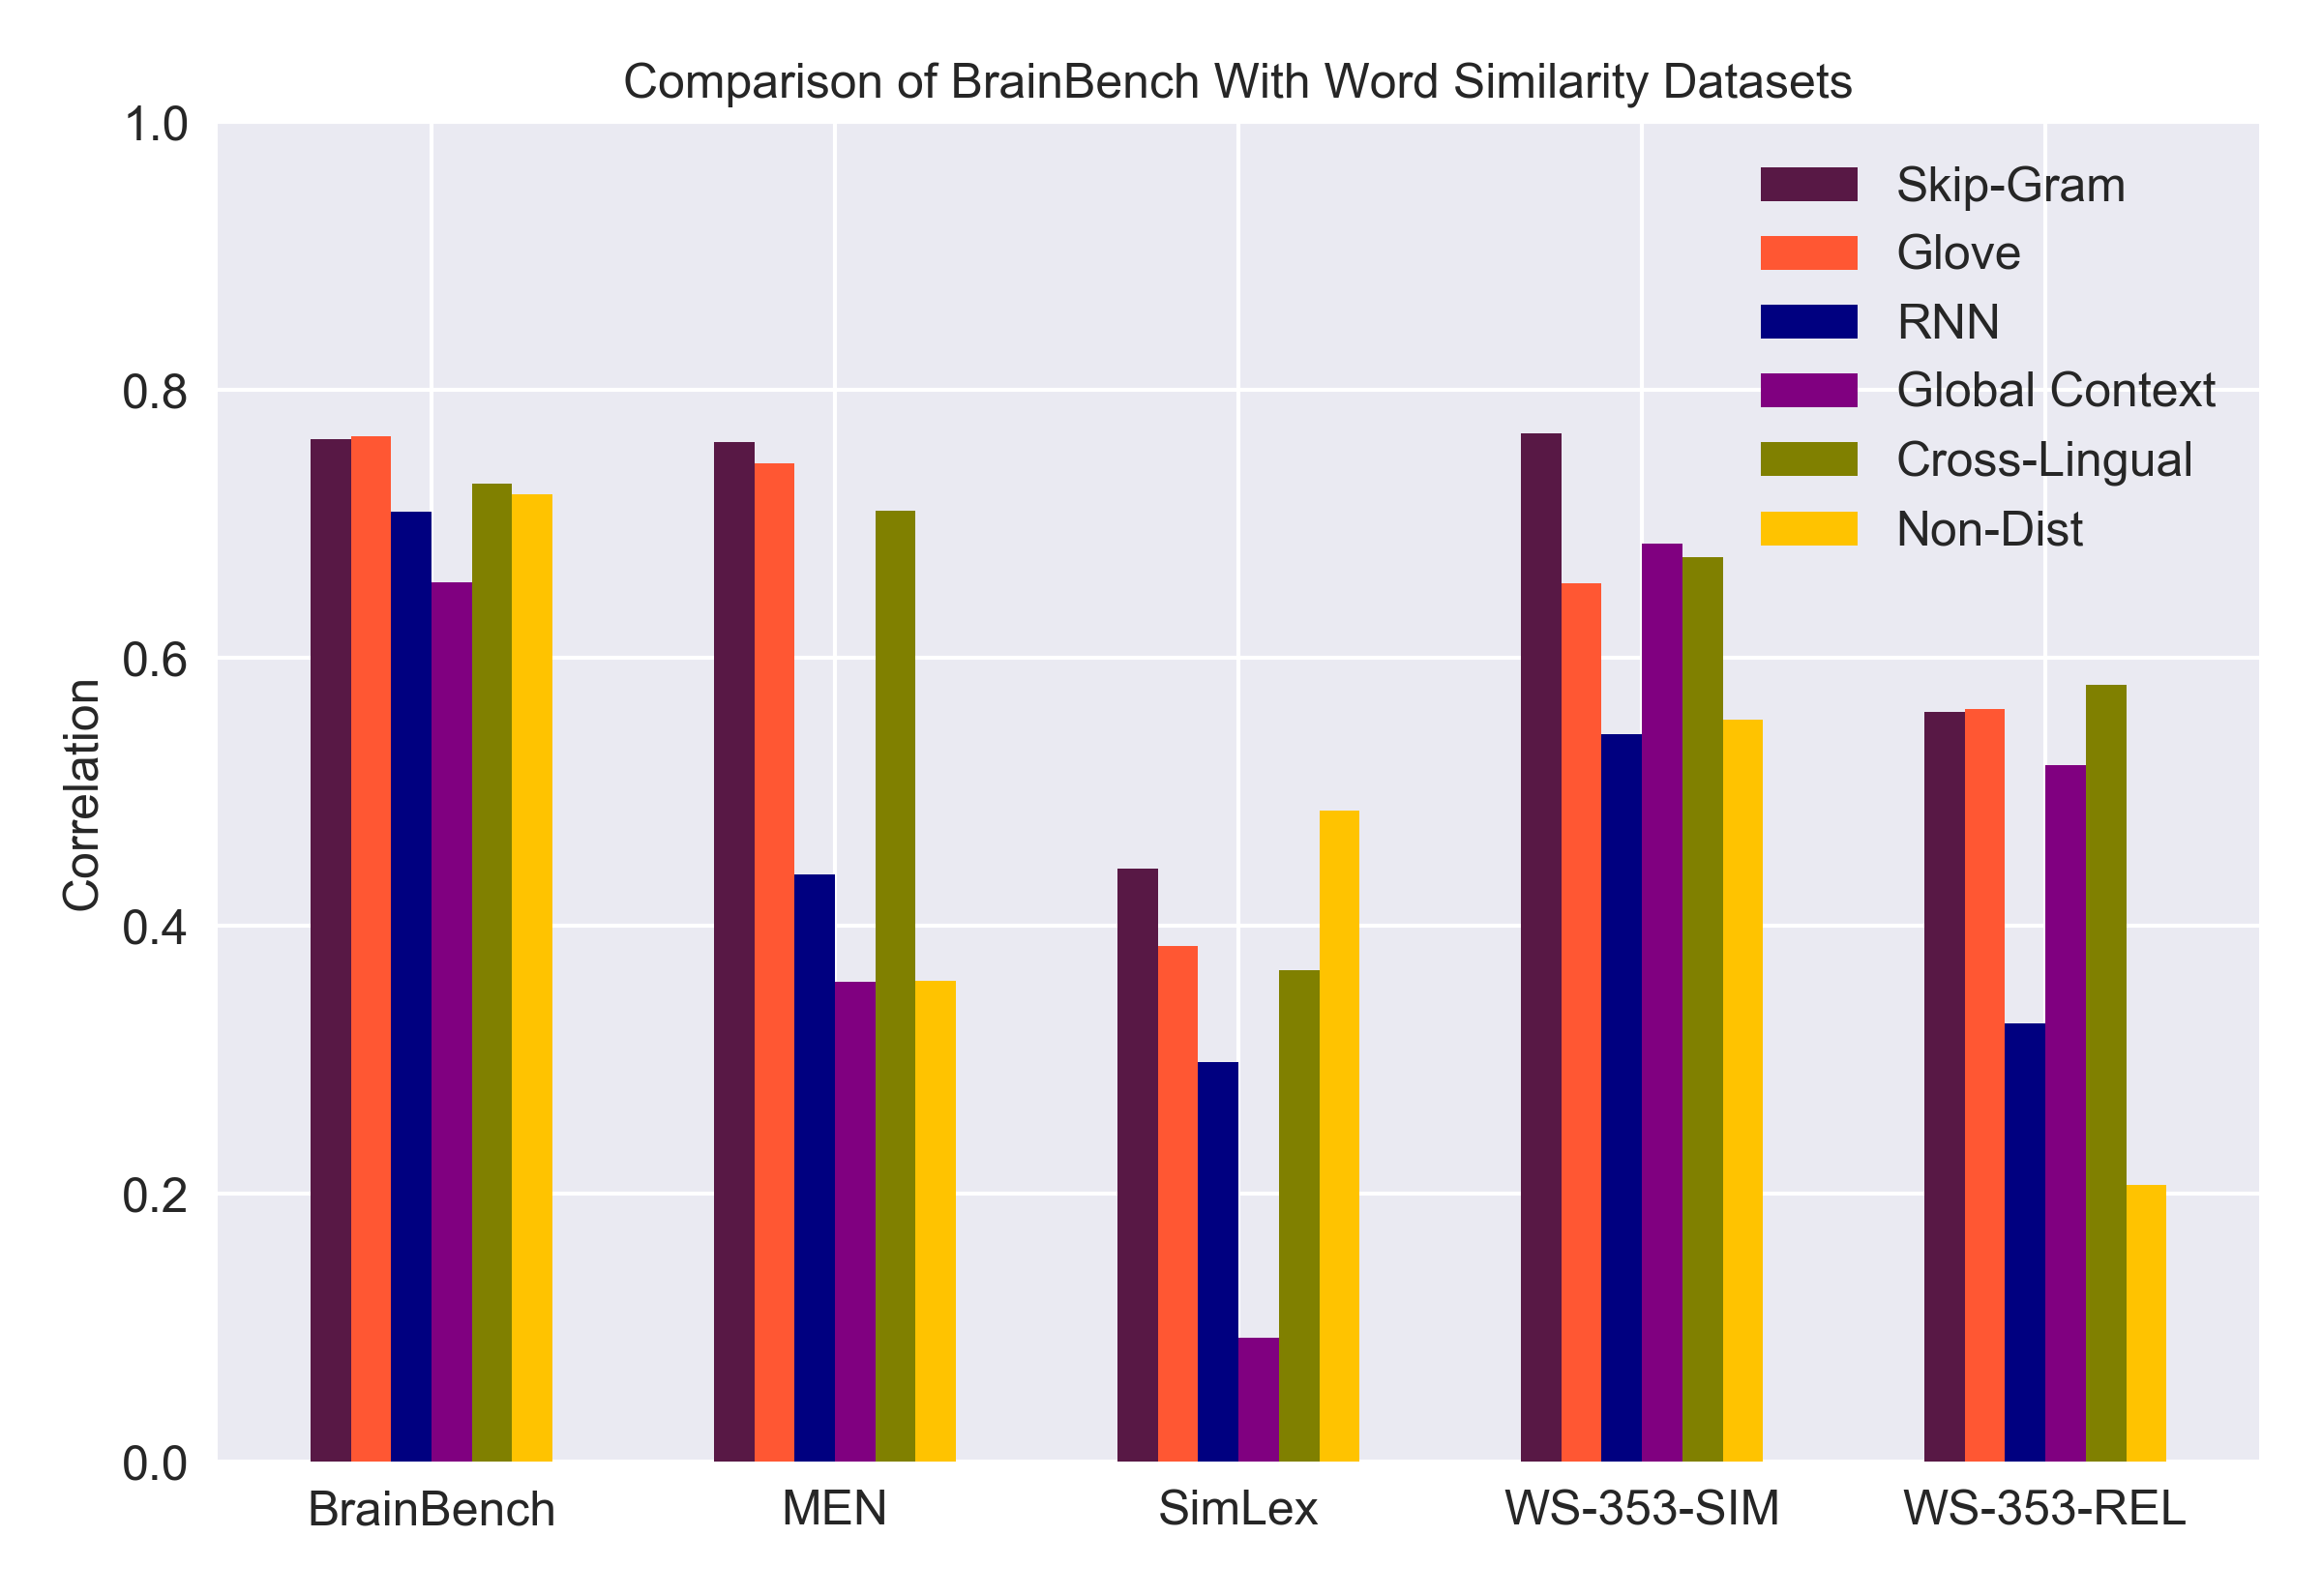
\includegraphics[width=14cm, height=9cm]{Figures/Comparison}
\caption{Comparison of BrainBench With Other Word Similarity Datasets}
\label{wordsimcomparison}
\end{figure}

We also compared the performance of the BrainBench with four other word similarity datasets. The similarity scores for MEN, SimLex, WS-353-SIM, and WS-353-REL, were obtained from Xu et al., 2016~\cite{BrainBench2016}.

Based on the correlation scores, BrainBench performs as good as MEN and WS-353-SIM. BrainBench also performs significantly better than SimLex and WS-353-REL. Both Skip-gram and Glove are the top performing DS models in both MEN and BrainBench. However, the performance of RNN, Global Context and Non-Distributional models are significantly lower in all the similarity datasets as compared to BrainBench. Compared to BrainBench, WS-SIM-353 dataset has better performance for Global Context vectors. 

The performance of BrainBench differs from previous benchmarks, implying that the BrainBench may test for a kind of semantic information which is not readily available in behavioral data.

%Compare BrainBench versions.
\subsection{2 vs. 2 accuracies for DS models against Anatomical ROIs in human brain}




%===========================================================
%Talk about Anatomical Brain Regions.

The voxels from the fMRI data collected by Mitchell et al., 2008 were mapped to the anatomical regions of the brain using the MNI template~\cite{Mitchell1191}. There were more than 120 regions of interest (ROI) identified in the original fMRI data across all nine participants. However, we included only those regions which had at least 200 voxels in each of the nine participants. 43 such ROIs were filtered out using this criterion. 
\begin{figure}[!t]
\centering
%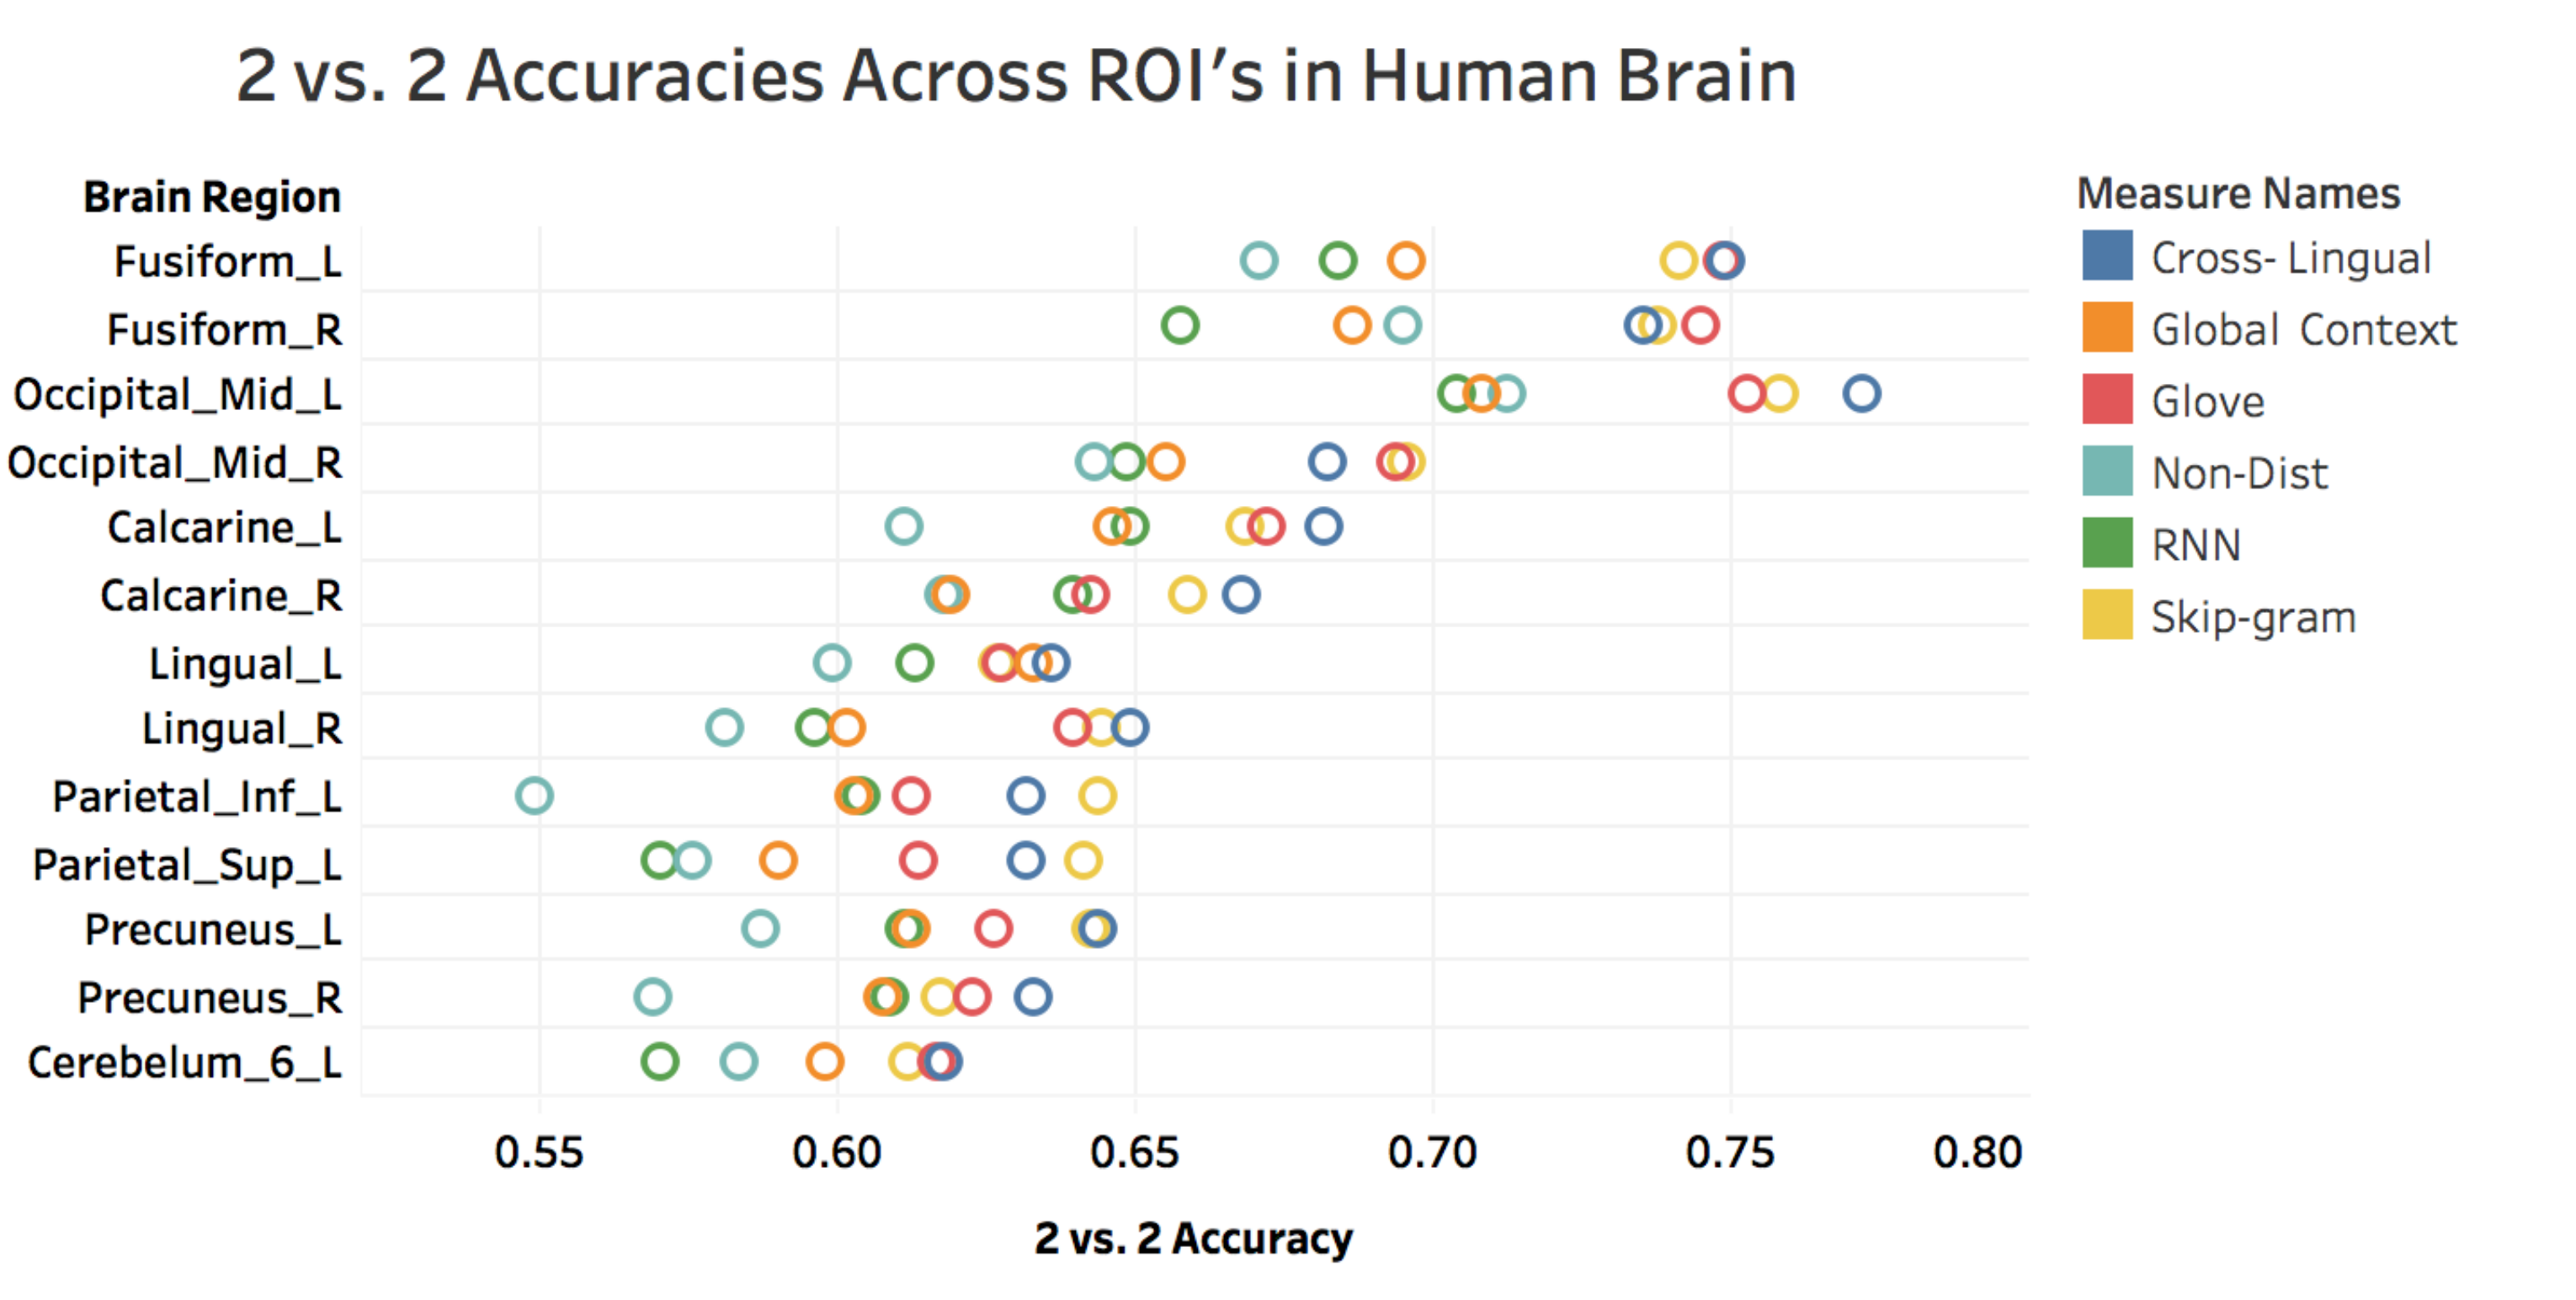
\includegraphics[width=12cm, height=6cm]{Figures/c}
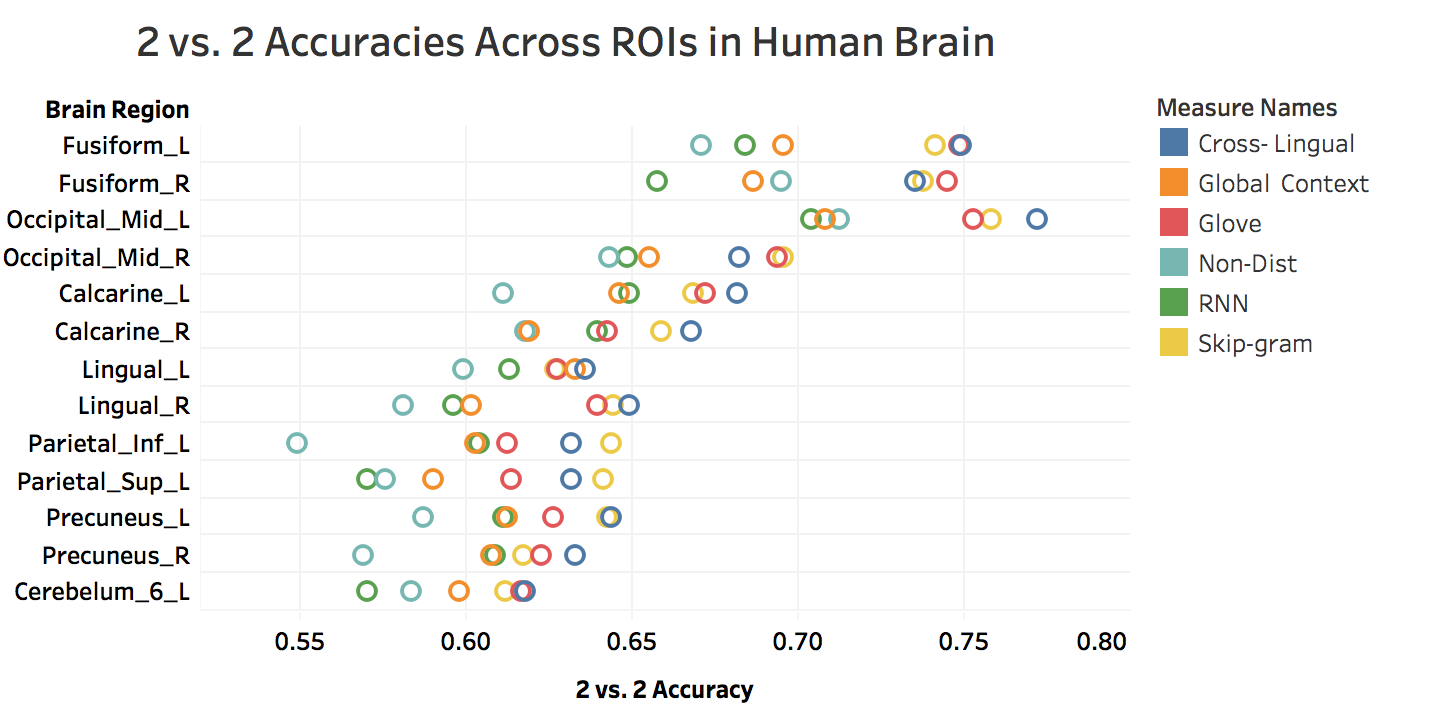
\includegraphics[width=12cm, height=6cm]{Figures/temp1}
\caption{Performance of DS models against various ROIs in brain.}
\label{roi}
\end{figure}
After removing the visual features from the brain data, we extracted the voxels corresponding to these 43 ROIs in the brain for the 60 concepts. This results in $60*v$ matrix for every anatomical region that we were included in our experiments. Here $v$ is again the number of voxels. We then computed the Pearson correlation to generate our brain correlation matrix $C_B$. Similarly, $C_D$  represents the correlation matrix corresponding to a DS model. Then the 2 vs. 2 tests are conducted for every ROI and DS pairs. This is followed by permutations tests to determine the statistical significance of the tests. We only report 13 top performing ROIs in our results. The results are summarized in Figure:~\ref{roi}.

The high performing ROIs included both the fusiform gyrus, and occipital lobe. The fusiform gyrus which forms the part of both occipital and temporal lobe of the brain is the top performing ROI, along with the medial surface of the left occipital lobe. Fusiform gyrus is part of the linguistics processing area of the brain and is known to take part in word recognition (contains word-form area)~\cite{nobre1994word}. Fusiform gyrus is also generally associated with face and body part stimuli. The occipital lobe is the visual processing in the brain and involved in decoding semantics from visual imagery. Skip-gram, Glove and Cross-Lingual performs considerably better as compared to RNN, Non-Distributional and Global-Context in both the fusiform gyrus and the Occipital lobes.

The calcarine sulcus and Lingual regions achieve intermediate performance with an average 2 vs. 2 accuracy of $0.65$ for all the 6 word vectors. The calcarine region is associated with the visual processing whereas Lingual regions have been shown to take part in both visual and word processing~\cite{andersonBrainEyes}. The 2 vs. 2 accuracies for all DS models were found to be statistically significant for both these regions ($p<0.01$).


The inferior and superior left parietal lobe, the left and right precuneus and the left cerebellum regions show the worst performance. In fact, Non-Distributional, Global-context and RNN fail to pass the significance threshold of p=0.05. It should be noted that these regions are not primarily associated with either linguistic or visual processing in the brain which might explain the poor performance of DS models in these regions. On average the Non-Distributed model which  is the worst performing model across all the anatomical brain region. Cross-Lingual, on the other hand, is the best performing DS model. The summary of the performance of all the 6 DS models against all the 43 ROIs could be found in Figure:\ref{all43} in appendix~\ref{chapter:appendix}.

The results described in this section could help the linguistics community studying language and visual representation in the human brain. There seems to be a large variation in the performance of various DS across anatomical brain regions, and our results could be used by researchers as a guideline in selecting the appropriate word vectors to decode semantics in their brain related experiments. For example, a researcher studying visual processing areas in the brain could use Cross-lingual vectors to decode emergence of visual semantics in the brain. Cross-lingual have been shown by our results to perform the best in areas related to visual processing. Similarity Glove could be ideal for studies focused on language centers of the brain.




\subsection{Comparing BrainBench $v_{1.0}$ vs $v_{2.0}$}

The addition of Italian fMRI and EEG dataset is one of the most important contributions of this work. The initial version of BrainBench had only 60 nouns words from English fMRI and MEG brain data sources. We evaluated the Italian Skip-gram word vector against the Italian fMRI dataset and found performance comparable to its English version. The results could imply that brain datasets could be used to evaluate word vectors trained from text corpora of different languages and is independent of the native language of the participants from whom the brain data was collected. Moreover, the Italian fMRI dataset added to BrainBench $V_{2.0}$ has a small coverage of abstract words (40 words) as compared to none in its first iteration.

Prior research has shown that the performance of abstract concepts on semantic tasks is lower than concrete concepts~\cite{AndersonConcreteness}. Despite of the newly added abstract words in BrainBench  $V_{2.0}$, the performance of our tool is comparable to other word similarity task datasets.

\begin{figure}[t]
\centering
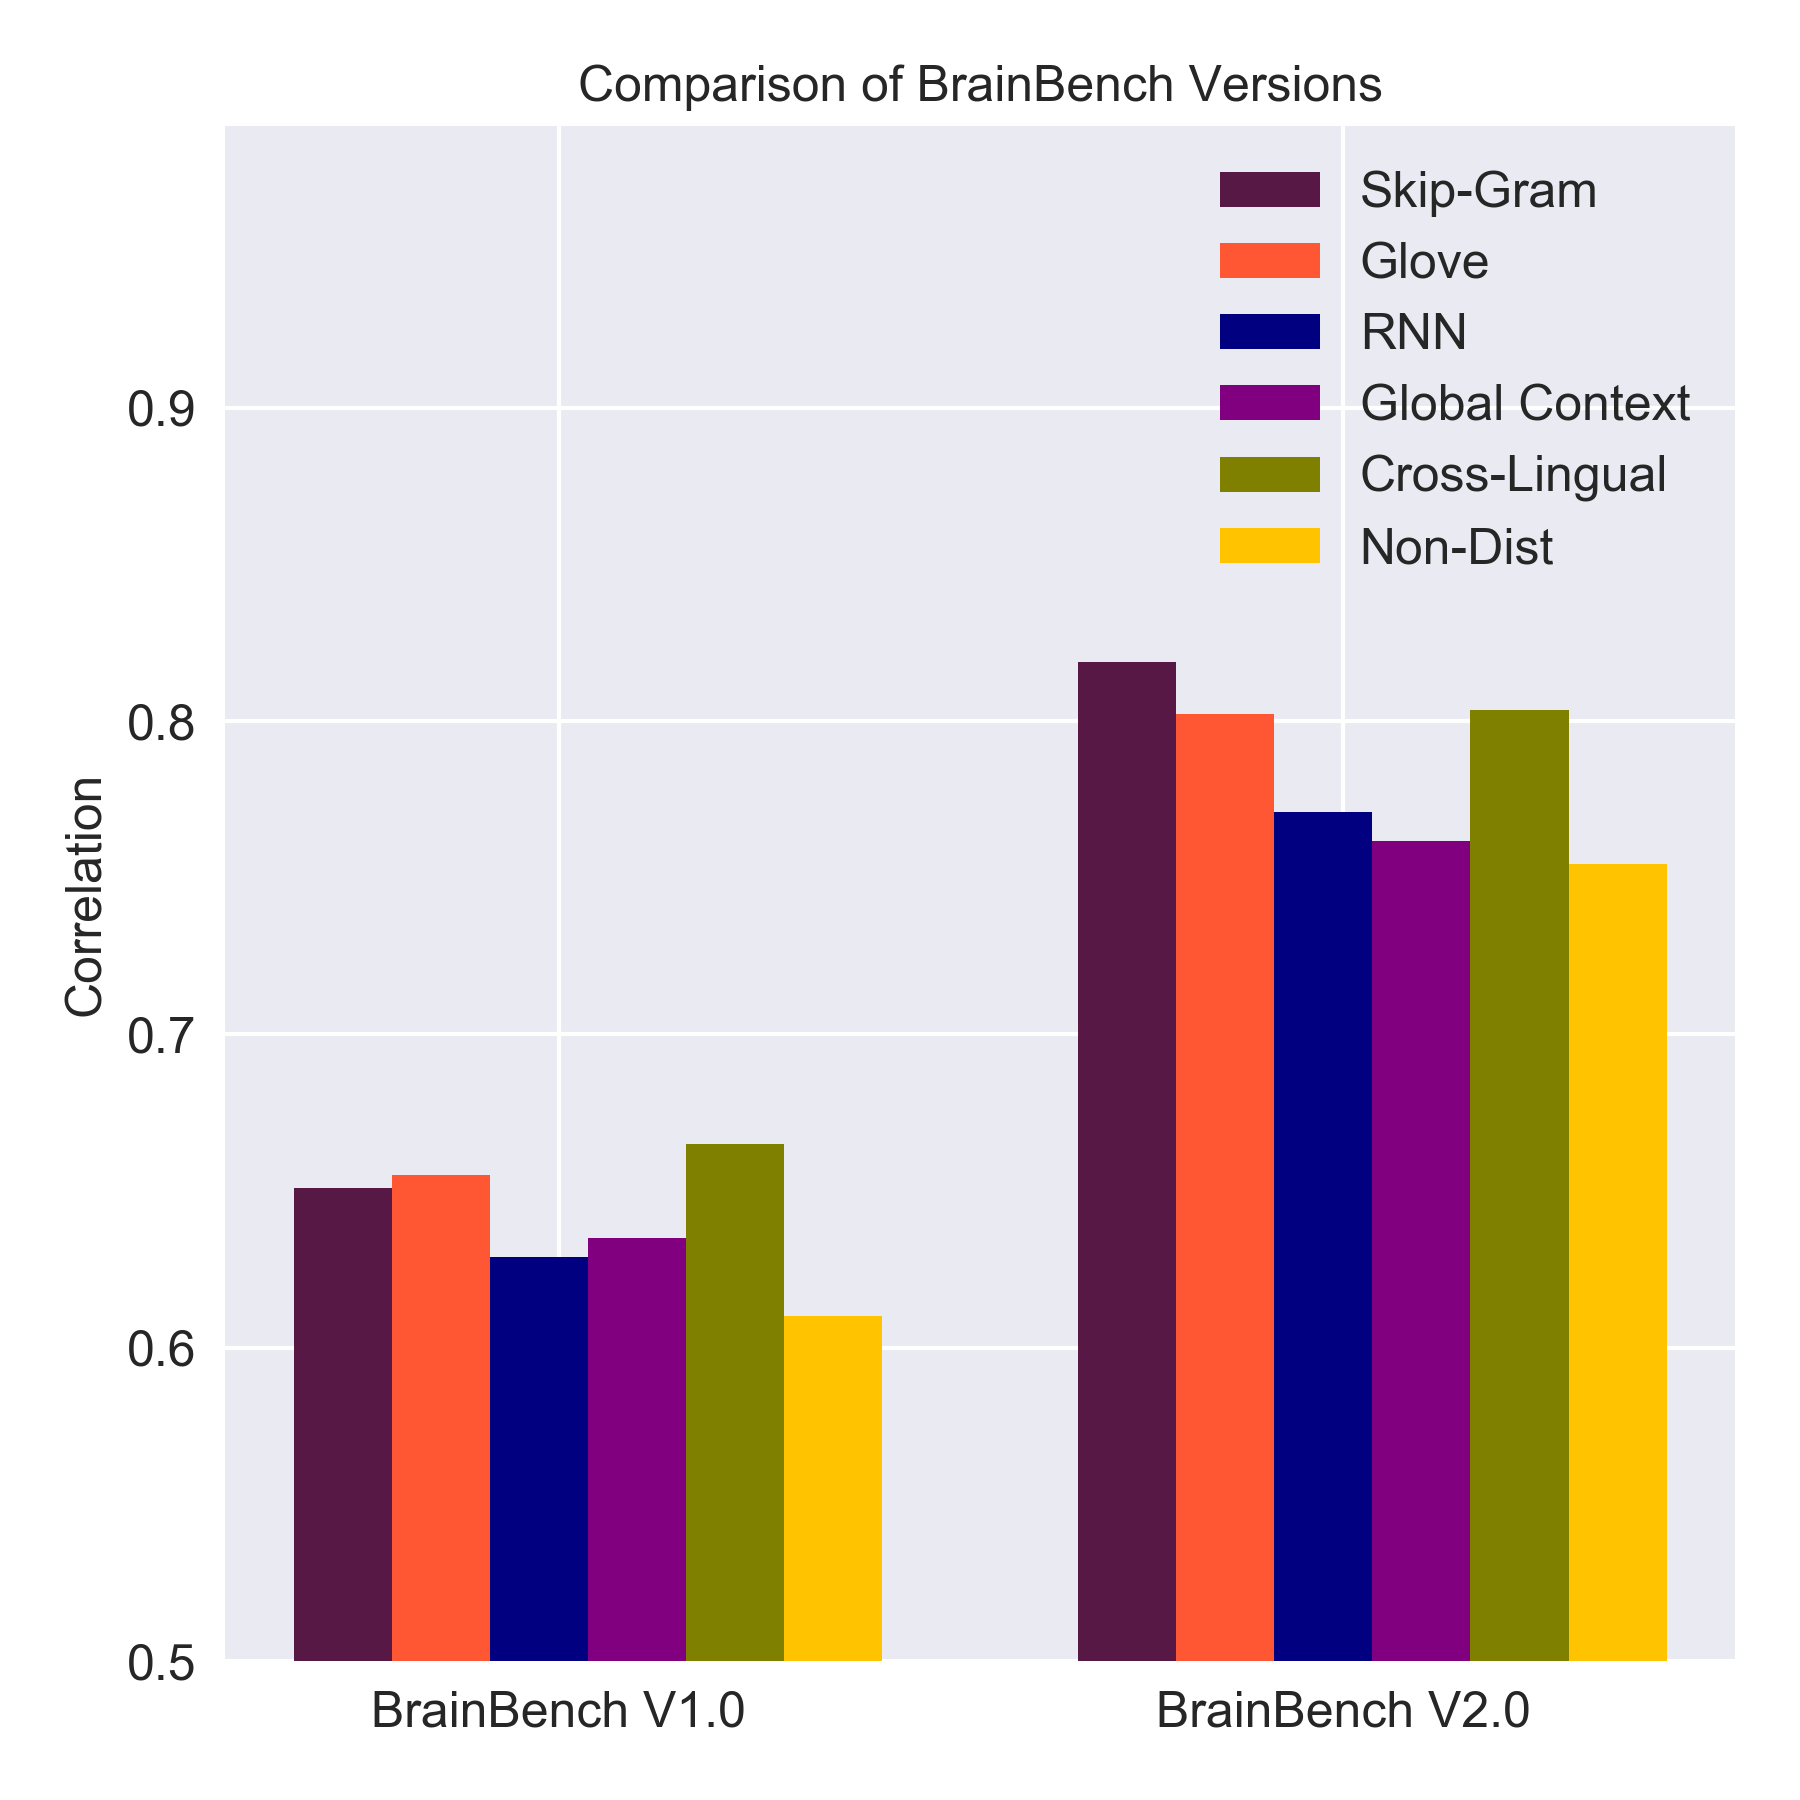
\includegraphics[width=12cm, height=11cm]{Figures/Versions}
\caption{Comparison of BrainBench $v_{1.0}$ vs $v_{2.0}$ Test Results}
\label{versions}
\end{figure}
The fMRI and MEG dataset were part of the first iteration of BrainBench. The reason that we decided to include these datasets is that we have changed the methodology associated with the BrainBench. In the first iteration by Xu et al., 2016 voxel selection was performed before removing visual features from the Brain datasets. In this work, we have reversed the order with visual features being removed before voxel selection. This small change in methodology does have a significant impact on the results. In Figure:~\ref{versions} we have compared the performance of both the versions of BrainBench. It should be noted that the results are based on the average of fMRI and MEG scores only (EEG and Italian fMRI are not included to keep the comparison fair).

Voxel selection selects the most stable voxels and helps to remove noise from the signal. However, if voxel selection is performed without removing visual features from the signal, the most stable voxels selected could be the ones which are correlated with visual features rather than semantics. Therefore, in our methodology visual features were removed from the signal before voxel selection.

Another contribution of this work is the study of the performance of various DS models against anatomical regions of interest (ROIs) in brain. The voxels corresponding to various anatomical brain regions were isolated, and separate 2 vs. 2 tests were executed against various DS models. We found that Cross-Lingual, Skip-gram and Glove perform the best across various linguistic and visual processing areas in the human brain.

\section{Summary}

This chapter focused on addressing the contributions made in improving the BrainBench tool designed to evaluate and benchmark word vectors (Contribution A). The preliminaries, which include both the brain datasets and the DS models used in our experiments along with the methodology used, were discussed in this chapter. We also discussed and compared our results with the previous iteration of BrainBench released in 2016. This thesis has extended the coverage of BrainBench from 60 concrete nouns from 2 brain datasets to 190 nouns (30 Abstract) from 4 brain datasets. Some key contributions here include the addition of Italian language datasets which includes an EEG sourced dataset. We also found that DS models show a high correlation to EEG brain signals. We also compared the performance of BrainBench with other word similarity datasets and found comparable performance measures. Finally, we studied the performance of DS models against anatomical brain regions and found that some DS models show correlation with brain regions associated with language and visual processing.





